% Options for packages loaded elsewhere
\PassOptionsToPackage{unicode}{hyperref}
\PassOptionsToPackage{hyphens}{url}
%
\documentclass[
  12pt,
]{article}
\title{\textbf{Appendix}}
\usepackage{etoolbox}
\makeatletter
\providecommand{\subtitle}[1]{% add subtitle to \maketitle
  \apptocmd{\@title}{\par {\large #1 \par}}{}{}
}
\makeatother
\subtitle{\textbf{Effect of Tocilizumab, Sarilumab, and Baricitinib on
Mortality Among Patients Hospitalized for COVID-19 Treated with
Corticosteroids: A Systematic Review and Meta-Regression}}
\author{}
\date{\vspace{-2.5em}}

\usepackage{amsmath,amssymb}
\usepackage{lmodern}
\usepackage{iftex}
\ifPDFTeX
  \usepackage[T1]{fontenc}
  \usepackage[utf8]{inputenc}
  \usepackage{textcomp} % provide euro and other symbols
\else % if luatex or xetex
  \usepackage{unicode-math}
  \defaultfontfeatures{Scale=MatchLowercase}
  \defaultfontfeatures[\rmfamily]{Ligatures=TeX,Scale=1}
\fi
% Use upquote if available, for straight quotes in verbatim environments
\IfFileExists{upquote.sty}{\usepackage{upquote}}{}
\IfFileExists{microtype.sty}{% use microtype if available
  \usepackage[]{microtype}
  \UseMicrotypeSet[protrusion]{basicmath} % disable protrusion for tt fonts
}{}
\makeatletter
\@ifundefined{KOMAClassName}{% if non-KOMA class
  \IfFileExists{parskip.sty}{%
    \usepackage{parskip}
  }{% else
    \setlength{\parindent}{0pt}
    \setlength{\parskip}{6pt plus 2pt minus 1pt}}
}{% if KOMA class
  \KOMAoptions{parskip=half}}
\makeatother
\usepackage{xcolor}
\IfFileExists{xurl.sty}{\usepackage{xurl}}{} % add URL line breaks if available
\IfFileExists{bookmark.sty}{\usepackage{bookmark}}{\usepackage{hyperref}}
\hypersetup{
  pdftitle={Appendix},
  hidelinks,
  pdfcreator={LaTeX via pandoc}}
\urlstyle{same} % disable monospaced font for URLs
\usepackage[margin=1in]{geometry}
\usepackage{graphicx}
\makeatletter
\def\maxwidth{\ifdim\Gin@nat@width>\linewidth\linewidth\else\Gin@nat@width\fi}
\def\maxheight{\ifdim\Gin@nat@height>\textheight\textheight\else\Gin@nat@height\fi}
\makeatother
% Scale images if necessary, so that they will not overflow the page
% margins by default, and it is still possible to overwrite the defaults
% using explicit options in \includegraphics[width, height, ...]{}
\setkeys{Gin}{width=\maxwidth,height=\maxheight,keepaspectratio}
% Set default figure placement to htbp
\makeatletter
\def\fps@figure{htbp}
\makeatother
\setlength{\emergencystretch}{3em} % prevent overfull lines
\providecommand{\tightlist}{%
  \setlength{\itemsep}{0pt}\setlength{\parskip}{0pt}}
\setcounter{secnumdepth}{-\maxdimen} % remove section numbering
\newlength{\cslhangindent}
\setlength{\cslhangindent}{1.5em}
\newlength{\csllabelwidth}
\setlength{\csllabelwidth}{3em}
\newlength{\cslentryspacingunit} % times entry-spacing
\setlength{\cslentryspacingunit}{\parskip}
\newenvironment{CSLReferences}[2] % #1 hanging-ident, #2 entry spacing
 {% don't indent paragraphs
  \setlength{\parindent}{0pt}
  % turn on hanging indent if param 1 is 1
  \ifodd #1
  \let\oldpar\par
  \def\par{\hangindent=\cslhangindent\oldpar}
  \fi
  % set entry spacing
  \setlength{\parskip}{#2\cslentryspacingunit}
 }%
 {}
\usepackage{calc}
\newcommand{\CSLBlock}[1]{#1\hfill\break}
\newcommand{\CSLLeftMargin}[1]{\parbox[t]{\csllabelwidth}{#1}}
\newcommand{\CSLRightInline}[1]{\parbox[t]{\linewidth - \csllabelwidth}{#1}\break}
\newcommand{\CSLIndent}[1]{\hspace{\cslhangindent}#1}
\usepackage{titling}
\pretitle{\begin{center}\huge\bfseries}
\posttitle{\end{center}}
\usepackage{pdflscape}
\newcommand{\blandscape}{\begin{landscape}}
\newcommand{\elandscape}{\end{landscape}}
\usepackage{geometry}
\usepackage{authblk}
\author[1]{Arthur M. Albuquerque}
\author[2]{Igor Eckert BS}
\author[3]{Lucas Tramujas MD}
\author[4,5]{Guillaume Butler-Laporte MD}
\author[6,7]{Emily G. McDonald MD MSc}
\author[5,8]{James M. Brophy MD PhD}
\author[4,5,6]{Todd C. Lee MD MPH}
\affil[1]{\small School of Medicine, Universidade Federal do Rio de Janeiro, Brazil}
\affil[2]{Department of Nutrition, Universidade Federal de Ciências da Saúde de Porto Alegre, Brazil}
\affil[3]{HCor Research Institute, Brazil}
\affil[4]{Division of Infectious Diseases, Department of Medicine, McGill University, Canada}
\affil[5]{Department of Epidemiology, Occupational Health, and Biostatistics, McGill University, Canada}
\affil[6]{Clinical Practice Assessment Unit, Department of Medicine, McGill University, Canada}
\affil[7]{Division of General Internal Medicine, Department of Medicine, McGill University, Canada}
\affil[8]{Division of Cardiology, Department of Medicine, McGill University, Canada}
\renewcommand\contentsname{Table of Contents}
\usepackage{booktabs}
\usepackage{longtable}
\usepackage{array}
\usepackage{multirow}
\usepackage{wrapfig}
\usepackage{float}
\usepackage{colortbl}
\usepackage{pdflscape}
\usepackage{tabu}
\usepackage{threeparttable}
\usepackage{threeparttablex}
\usepackage[normalem]{ulem}
\usepackage{makecell}
\usepackage{xcolor}
\usepackage{amsmath}
\usepackage{caption}
\ifLuaTeX
  \usepackage{selnolig}  % disable illegal ligatures
\fi

\begin{document}
\maketitle

\newpage 
\tableofcontents 
\newpage

\hypertarget{appendix-methods}{%
\section{Appendix Methods}\label{appendix-methods}}

\hypertarget{search-strategies}{%
\subsection{Search Strategies}\label{search-strategies}}

\textbf{PubMed:}

\begingroup\fontsize{9.3}{11.3}\selectfont

\begin{tabu} to \linewidth {>{\raggedright}X>{\raggedright}X}
\hline
Query & Terms\\
\hline
\cellcolor{gray!6}{\#1} & \cellcolor{gray!6}{(randomized controlled trial[pt] OR controlled clinical trial[pt] OR randomized[tiab] OR placebo[tiab] OR drug therapy[sh] OR randomly[tiab] OR trial[tiab] OR groups[tiab] NOT (animals [mh] NOT humans [mh]))}\\
\hline
\#2 & coronavirus[Title] OR "corona virus" [Title] OR "corona pandemic"[Title] OR coronavirinae[Title] OR coronaviridae[Title] OR betacoronavirus[Title] OR covid19[Title] OR covid[Title] OR nCoV[Title] OR "CoV 2"[Title] OR CoV2[Title] OR sars2[Title] OR sarscov2[Title] OR 2019nCoV[Title] OR "novel CoV"[Title] OR "wuhan virus"[Title] OR coronavirus[Title/Abstract] OR "corona virus" [Title/Abstract] OR "corona pandemic"[Title/Abstract] OR coronavirinae[Title/Abstract] OR coronaviridae[Title/Abstract] OR betacoronavirus[Title/Abstract] OR covid19[Title/Abstract] OR covid[Title/Abstract] OR nCoV[Title/Abstract] OR "CoV 2"[Title/Abstract] OR CoV2[Title/Abstract] OR sars2[Title/Abstract] OR sarscov2[Title/Abstract] OR 2019nCoV[Title/Abstract] OR "novel CoV"[Title/Abstract] OR "wuhan virus"[Title/Abstract] OR "COVID-19" [Appendix Concept] OR "severe acute respiratory syndrome coronavirus 2" [Appendix Concept] OR ((wuhan[Title] OR hubei[Title] OR huanan[Title]) OR (wuhan[Title/Abstract] OR hubei[Title/Abstract] OR huanan[Title/Abstract]) AND ("severe acute respiratory"[Title] OR pneumonia[Title])) OR (("severe acute respiratory"[Title/Abstract] OR pneumonia[Title/Abstract]) AND (outbreak[Title]) OR outbreak[Title/Abstract])\\
\hline
\cellcolor{gray!6}{\#3} & \cellcolor{gray!6}{sarilumab[Title/Abstract]}\\
\hline
\#4 & baricitinib[Title/Abstract]\\
\hline
\cellcolor{gray!6}{\#5} & \cellcolor{gray!6}{tocilizumab[Title/Abstract]}\\
\hline
\end{tabu}
\endgroup{}

Tocilizumab: \#1 AND \#2 AND \#5

Sarilumab: \#1 AND \#2 AND \#3

Baricitinib: \#1 AND \#2 AND \#4

\newpage

\textbf{CENTRAL:}

\begin{table}[!h]
\centering
\begin{tabular}[t]{l|l}
\hline
Query & Terms\\
\hline
\#1 & MeSH descriptor: [COVID-19] explode all trees\\
\hline
\#2 & sarilumab with PubYear from 2021 to 2021, in Trials\\
\hline
\#3 & baricitinib\\
\hline
\#4 & tocilizumab with PubYear from 2021 to 2021, in Trials\\
\hline
\end{tabular}
\end{table}

Tocilizumab: \#1 AND \#4

Sarilumab: \#1 AND \#2

Baricitinib: \#1 AND \#3

\textbf{EMBASE:}

\begin{tabu} to \linewidth {>{\raggedright}X>{\raggedright}X}
\hline
Query & Terms\\
\hline
\cellcolor{gray!6}{\#1} & \cellcolor{gray!6}{('crossover procedure'/exp OR 'crossover procedure') AND [embase]/lim OR (('prospective study'/exp OR 'prospective study') AND [embase]/lim) OR (('follow up'/exp OR 'follow up') AND [embase]/lim) OR (('placebo'/exp OR 'placebo') AND [embase]/lim) OR (('clinical trial'/exp OR 'clinical trial') AND [embase]/lim) OR (('single blind procedure'/exp OR 'single blind procedure') AND [embase]/lim) OR (('double blind procedure'/exp OR 'double blind procedure') AND [embase]/lim) OR (('randomization'/exp OR 'randomization') AND [embase]/lim) OR (('controlled clinical trial'/exp OR 'controlled clinical trial') AND [embase]/lim) OR (('randomized controlled trial'/exp OR 'randomized controlled trial') AND [embase]/lim)}\\
\hline
\#2 & baricitinib':ti,ab\\
\hline
\cellcolor{gray!6}{\#3} & \cellcolor{gray!6}{sarilumab':ti,ab}\\
\hline
\#4 & tocilizumab':ti,ab\\
\hline
\cellcolor{gray!6}{\#5} & \cellcolor{gray!6}{coronavirus infection' OR 'coronavirus disease 2019' OR 'severe acute respiratory syndrome coronavirus 2'}\\
\hline
\end{tabu}

Tocilizumab: \#1 AND \#4 AND \#5 AND 2021:py

Sarilumab: \#1 AND \#3 AND \#5 AND 2021:py

Baricitinib: \#1 AND \#2 AND \#5

\newpage

\textbf{Medrxiv:}

\begin{tabu} to \linewidth {>{\raggedright}X>{\raggedright}X}
\hline
Query & Terms\\
\hline
\cellcolor{gray!6}{\#1} & \cellcolor{gray!6}{(sarilumab OR baricitinib OR tocilizumab) AND (covid-19 OR coronavirus OR covid) AND random*" and abstract or title "random randomized randomly randomised placebo-controlled}\\
\hline
\end{tabu}

\newpage

\hypertarget{data-synthesis-and-analysis}{%
\subsection{Data Synthesis and
Analysis}\label{data-synthesis-and-analysis}}

\hypertarget{meta-analysis}{%
\subsubsection{Meta-analysis}\label{meta-analysis}}

For each set of studies (tocilizumab, baricitinib, or sarilumab
vs.~control), we fitted a Bayesian random-effects meta-analysis. Each
model is defined as:

\begin{align*}
y_i & \sim Normal(\theta_i, \sigma_i^2)\\
\theta_i & \sim Normal(\mu, \tau^2)\\
\end{align*}

where \(y_i\) is the observed mean log odds ratio in study \(i\) for
either tocilizumab, sarilumab, or baricitinib versus control treatment.
We assume these effect sizes are normally distributed around the
study-specific mean \(\theta_i\) along with a known sampling variance,
represented by the observed \(\sigma_i^2\). We also assume \(\theta_i\)
is drawn from a normal distribution where \(\mu\) is the average effect
and \(\tau^2\) is the between-study heterogeneity.

Because these are Bayesian models, we need to specify prior
distributions for all parameters. We applied a prior for \(\mu\) that
cover plausible values, assigning limited density to unlikely values,
and thereby exerting little influence on the results in all models. A
simulation study supported by empirical evidence suggests that a prior
with a 95\% interval between \(0.23\) and \(4.35\) is suitable to this
case.(\protect\hyperlink{ref-pedroza2018}{1}) In the log scale, such
prior is described as:

\begin{align*}
\mu & \sim \operatorname{Normal}(0, 0.75^2)
\end{align*}

\begin{center}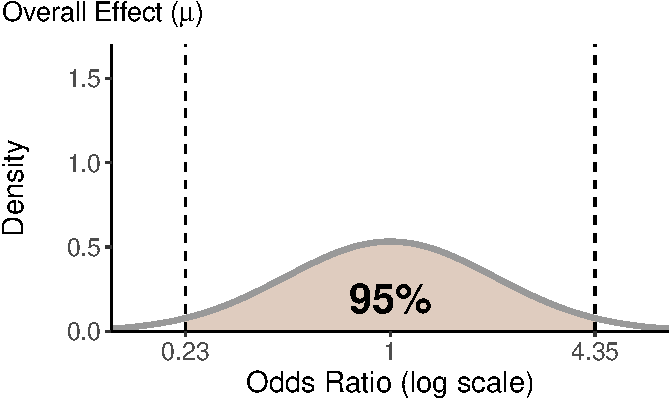
\includegraphics{supplementary_material_files/figure-latex/mu prior visualization-1} \end{center}

\newpage

Regarding the between-study standard deviation parameter (\(\tau\)), we
used an informative prior based on previous evidence. We applied the
predictive distribution on all-cause mortality for ``placebo / control''
vs.~``pharmacological'' comparisons derived by Turner et
al.(\protect\hyperlink{ref-turner2015}{2})

Although the definition of small or large between-study heterogeneity is
arbitrary, previous work suggests cutoff values (``reasonable''
heterogeneity between 0.1 and 0.5, and ``fairly high'' between 0.5 and
1.0.(\protect\hyperlink{ref-spiegelhalter2004}{3}) We added a category
for low heterogeneity (between 0 and 0.1):

\begin{align*}
\tau & \sim \operatorname{Log-Normal}(-1.975, 0.67^2)
\end{align*}

\begin{center}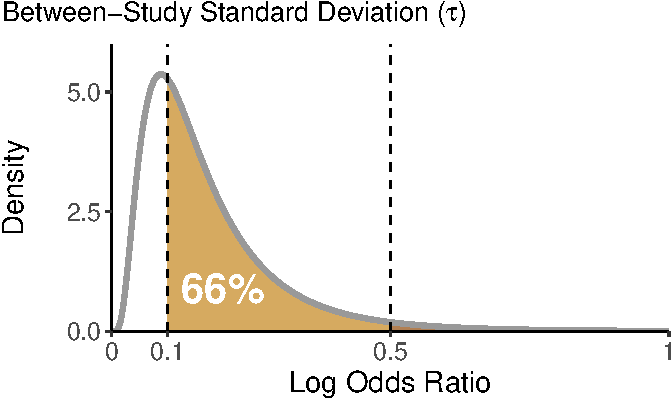
\includegraphics{supplementary_material_files/figure-latex/informative tau prior visualization-1} \end{center}

This distribution concentrates 31\% of probability density between 0 and
0.1 log odds ratio (`low heterogeneity'), 66\% between 0.1 and 0.5
(`reasonable'), and only 4\% between 0.5 and 1.0 (`fairly high').

\newpage

While maintaining the same prior for \(\mu\), we added a post-hoc
sensitivity analysis using a less informative prior for
\(\tau\):(\protect\hyperlink{ref-rover2021}{4})

\begin{align*}
\tau & \sim \operatorname{Half-Normal}(0, 0.5^2)
\end{align*}

This distribution yields higher heterogeneity probabilities, while
limiting less plausible high levels.

\begin{center}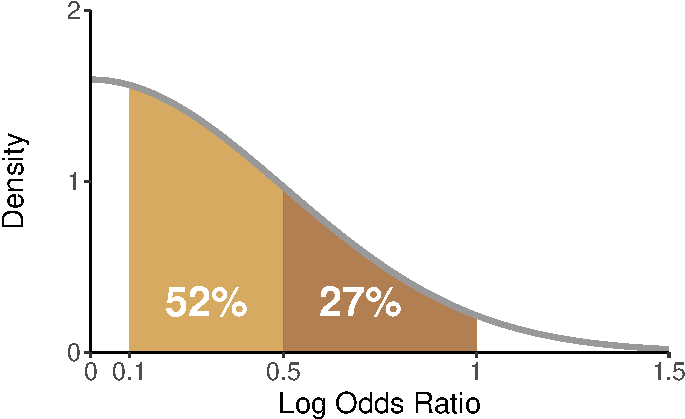
\includegraphics{supplementary_material_files/figure-latex/weakly tau prior visualization-1} \end{center}

This distribution concentrates 16\% of probability density between 0 and
0.1 log odds ratio (`low heterogeneity'), 52\% between 0.1 and 0.5
(`reasonable'), and 27\% between 0.5 and 1.0 (`fairly high').

\hypertarget{posterior-predictive-distribution}{%
\subsubsection{Posterior Predictive
Distribution}\label{posterior-predictive-distribution}}

To further explore the impact of between-study heterogeneity, we
evaluated the posterior predictive distribution in each meta-analysis.
This distribution allows inference about ``\ldots what we would expect
to see in a new study population that is exchangeable with the studies
included in our meta-analysis.''(\protect\hyperlink{ref-welton2020}{5})

\[\theta_{new} \sim \operatorname{Normal}(\mu, \tau^2)\]

The posterior predictive distribution estimates true treatment effects
(study populations, \(\theta_{new}\)) expected in future settings. This
distribution is vital to inform probable values for the true treatment
association in future settings, valuable for power calculations or prior
distribution elicitation in future
RCTs.(\protect\hyperlink{ref-spiegelhalter2004}{3}) This generates new
trial population parameter estimates, independently of sample size and
other population
characteristics.(\protect\hyperlink{ref-higgins2009}{6})

\hypertarget{meta-regression}{%
\subsubsection{Meta-regression}\label{meta-regression}}

Our primary research question is whether baricitinib and sarilumab are
noninferior to tocilizumab. A sensitive approach to answer this question
is to separately meta-analyze direct comparisons between tocilizumab
vs.~baricitinib and tocilizumab vs.~sarilumab. However, a preliminary
search by our research group showed a limited number of studies that
report such comparisons.(\protect\hyperlink{ref-zotero-3144}{7}) Thus,
we decided to only estimate the noninferiority probability of sarilumab
and baricitinib vs.~tocilizumab through indirect (across-trials)
comparisons. Because of the fragility of such comparisons, it is of
great interest to test the robustness of these estimates with multiple
prior distributions.

Bayesian network meta-analyses are historically used to estimate direct,
indirect, and mixed-effects when more than two treatment comparisons are
available.(\protect\hyperlink{ref-dias2018}{8}) However, this approach
does not allow one to assign prior distributions to specific comparisons
within the network, such as an indirect effect. To overcome this
limitation, we fitted Bayesian random-effect meta-regression models to
estimate the indirect differences mentioned above (two separate sets of
models: tocilizumab vs.~baricitinib; tocilizumab
vs.~sarilumab).(\protect\hyperlink{ref-pitchforth2012}{9}) These models
are identical to meta-regressions with a dichotomous covariate used to
evaluate subgroup differences.(\protect\hyperlink{ref-thompson2002}{10})
This approach allows one to apply a plethora of prior distributions
specifically to the indirect comparison between treatments.

Both baricitinib and sarilumab models are identical, and are described
as:(\protect\hyperlink{ref-pitchforth2012}{9})

\begin{align*}
y_i & \sim Normal(\theta_i, \sigma_i^2)\\
\theta_i & \sim Normal(\mu, \tau^2)\\
\mu &= \beta_0 + \beta_{1, T} x_i\\
\end{align*}

where \(y_i\) is the observed mean log odds ratio in study \(i\) for
either tocilizumab, sarilumab, or baricitinib versus control treatment.
We assume these effect sizes are normally distributed around the
study-specific mean \(\theta_i\) along with a known sampling variance,
represented by the observed \(\sigma_i^2\). We also assume \(\theta_i\)
is drawn from a normal distribution where \(\mu\) is the average effect
and \(\tau^2\) is the between-study heterogeneity. We will estimate
\(\mu\) as a function of the estimated population effect size
\(\beta_0\) and the moderator \(x\) multiplied by the coefficient
\(\beta_{1, T}\). \(x\) is dummy-coded, where \textbf{0} indicates that
the observed \(y_i\) is an effect size estimate of \textbf{tocilizumab}
compared to control, while \textbf{1} indicates that \(y_i\) is an
effect size estimate of the \textbf{sarilumab} (\(T = Sari\)) or
\textbf{baricitinib} (\(T = Bari\)) compared to control.

In summary, we can estimate the overall log odds ratio for tocilizumab,
sarilumab, and baricitinib (depending on which model) as:

\begin{itemize}
\tightlist
\item
  Tocilizumab = \(\beta_0\)
\item
  Sarilumab = \(\beta_0 + \beta_{1, Sari}\)
\item
  Baricitinib = \(\beta_0 + \beta_{1, Bari}\)
\end{itemize}

\(\beta_{1, T}\) is the parameter that estimates the indirect difference
between tocilizumab vs.~sarilumab or tocilizumab vs.~baricitinib. When
exponentiated, \(\beta_{1, T}\) yields the ratio of odds ratios, as
demonstrated below. We will reference sarilumab and baricitinib as
``comparator'' hereafter.

\begin{gather*}
\beta_{1, T}  = ln(OR_{comparator}) - ln(OR_{tocilizumab}) = ln(\frac{OR_{comparator}}{OR_{tocilizumab}})\\
exp(\beta_{1, T})  = \frac {OR_{comparator}}{OR_{tocilizumab}}
\end{gather*}

\hypertarget{priors}{%
\subsubsection{Priors}\label{priors}}

\(\beta_0\) represents the log odds ratio for tocilizumab vs.~control
(\(\ln[OR_{tocilizumab}]\)). Here, we applied the same prior mentioned
before (regarding \(\mu\)) for
\(\beta_0\):(\protect\hyperlink{ref-pedroza2018}{1})

\begin{align*}
\beta_0 & \sim \operatorname{Normal}(0, 0.75^2)
\end{align*}

Regarding the between-study standard deviation parameter (\(\tau\)), we
also used the same informative prior mentioned
before:(\protect\hyperlink{ref-turner2015}{2})

\begin{align*}
\tau & \sim \operatorname{Log-Normal}(-1.975, 0.67^2)
\end{align*}

In addition to the parameters mentioned above, we should also assign a
prior distribution for the indirect comparison parameter
(\(\beta_{1, T}\)). Inspired by the guidelines provided by Zampieri et
al.,(\protect\hyperlink{ref-zampieri2021}{11}) we fitted different
models to represent distinct beliefs. Before discussing these prior
distributions, we will first elucidate the underlying rationale of this
parameter.

A log odds ratio lower than \(0\) represents lower mortality in the
intervention arm (tocilizumab, sarilumab, or baricitinib) in comparison
to control. Moreover, the indirect comparison parameter represents the
absolute difference between comparator (sarilumab or baricitinib) and
tocilizumab studies in the log scale. Therefore, when the mortality
reduction due to intervention is greater in comparator studies (lower
\(\ln[OR_{comparator}]\) than \(ln[OR_{tocilizumab}]\)),
\(\beta_{1, T}\) is negative in the log scale:

\begin{align*}
\downarrow \ln(OR_{comparator}) - \uparrow \ln(OR_{tocilizumab}) \rightarrow -\beta_{1, T}\\
\end{align*}

Here is the same rationale in the linear scale to further facilitate
\(\beta_{1, T}\)'s prior elicitation:

\begin{align*}
exp(\beta_{1, T}) &= ROR =  \frac {OR_{comparator}}{OR_{tocilizumab}}
\end{align*}

where ROR is the ratio of odds ratios, i.e.~the interaction parameter
exponentiated (\(exp[\beta_{1, T}]\)). Thus, a ROR lower than \(1\) also
indicates greater mortality reduction due to intervention in comparator
studies:

\begin{align*}
\frac {\downarrow OR_{comparator}}{\uparrow OR_{tocilizumab}} \rightarrow ROR < 1
\end{align*}

We separately applied \(4\) normally distributed prior distributions for
\(\beta_{1, T}\) in each model (sarilumab and baricitinib's models),
which can be described based on the ``prior belief'' and ``belief
strength.'' While the former reflects the distribution's mean, the
latter reflects the distribution's standard deviation.

In the model comparing \textbf{sarilumab} to tocilizumab, the beliefs
are:

\begin{itemize}
\item
  ``Skeptical,'' which expects no difference between sarilumab and
  tocilizumab studies (mean centered at \(1\)) with \(95\%\) probability
  between \(0.5\) and \(2\) (linear scale, ratio of odds ratios). These
  values represent a weak belief
  strength,(\protect\hyperlink{ref-zampieri2021}{11}) based on the
  little information currently available on this topic.
  \(\operatorname{Normal}(0, 0.354^2)\)
\item
  ``Optimistic for Sarilumab,'' which expects a greater mortality
  reduction due to sarilumab use in comparison to tocilizumab. The mean
  is centered at \(0.952\) (linear scale, ratio of odds ratios), which
  was based on the single study that directly compared sarilumab to
  tocilizumab (REMAP-CAP).(\protect\hyperlink{ref-zotero-3144}{7}) In
  this study, they assessed ``hospital survival'' and an odds ratio
  greater than 1 indicated greater in-hospital mortality reduction due
  to sarilumab use in comparison to tocilzumab. As shown in their Figure
  S3, the median odds ratio of sarilumab vs.~tocilizumab was 1.05,
  indicating a greater odds of hospital survival due to sarilumab.
  However, in the present study, we will assess mortality (not hospital
  survival), and an odds ratio lower (not greater) than 1 represents
  greater mortality reduction due to sarilumab use. Thus, to guide this
  belief based on the study mentioned above, we calculated the
  reciprocal of 1.05 (\(1/1.05\)), which yields \(0.952\).
  \(\operatorname{Normal}(-0.049, 0.193^2)\)

  Further, we considered that there is 40\% of probability that the
  ratio of odds ratios is greater than \(1\). We chose 40\% because the
  single study that directly compared sarilumab to tocilizumab found
  34\% of probability density for tocilizumab's superiority over
  sarilumab.(\protect\hyperlink{ref-zotero-3144}{7}) However, this was
  the first and only study and therefore likely to be an over-estimate
  and not to include potential between study variability. We then
  elected to see a 40\% of probability for tocilizumab's superiority
  over sarilumab in this prior as being a ``realistic optimistic for
  Sarilumab'' prior.(\protect\hyperlink{ref-zotero-3144}{7}) Although
  not identical to the 30\% suggested by Zampieri et al.~-- which we
  consider too informative in this case, given that it would be more
  informative than the study mentioned above -- we believe this prior
  represents weak belief
  strength.(\protect\hyperlink{ref-zampieri2021}{11})
\item
  ``Optimistic for Tocilizumab,'' which expects a greater mortality
  reduction due to tocilizumab use in comparison to sarilumab. The mean
  is centered at \(1.05\), the reciprocal of \(0.952\). Similarly, this
  prior belief will also have a weak strength, represented by 40\% of
  probability that the ratio of odds ratios is lower than
  \(1\).(\protect\hyperlink{ref-zampieri2021}{11})
  \(\operatorname{Normal}(0.049, 0.193^2)\)
\item
  ``Vague,'' which represents no prior belief with no strength.
  \(\operatorname{Normal}(0, 4^2)\)
\end{itemize}

The first three distributions are shown below:

\begin{center}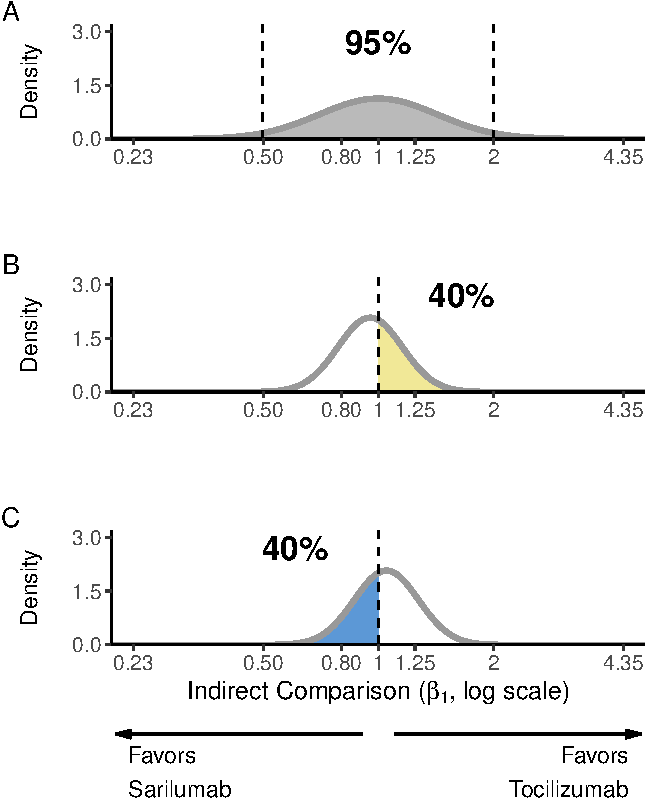
\includegraphics{supplementary_material_files/figure-latex/all priors sari meta regressions-1} \end{center}

Prior distributions for \(beta\_{1, Sari}\) (ratio of odds ratios) in
models comparing sarilumab to tocilizumab. Panel A: `Skeptical' prior.
The Normal(\(0\), \(0.354^2\)) distribution approximately concentrates
\(95\)\% of probability density between \(0.5\) and \(2.0\) in the
linear scale (\(-0.69\) and \(0.69\) in the log scale, respectively).
Panel B: `Optimistic for Sarilumab' prior. The Normal(\(-0.049\),
\(0.193^2\)) distribution approximately concentrates \(40\)\% of
probability density above \(1\). Panel C: `Optimistic for Tocilizumab'
prior. The Normal(\(0.049\), \(0.193^2\)) distribution approximately
concentrates \(40\)\% of probability density below \(1\).

\newpage

In the model comparing \textbf{baricitinib} to tocilizumab, the beliefs
are:

\begin{itemize}
\item
  ``Skeptical,'' which expects no difference between baricitinib and
  tocilizumab studies (mean centered at \(1\)) with \(95\%\) probability
  between \(0.5\) and \(2\) (linear scale, ratio of odds ratios). These
  values represent a weak belief
  strength,(\protect\hyperlink{ref-zampieri2021}{11}) based on the
  little information currently available on this topic.
  \(\operatorname{Normal}(0, 0.354^2)\)
\item
  ``Optimistic for Baricitinib,'' which expects a greater mortality
  reduction due to baricitinib use in comparison to tocilizumab. The
  mean is centered at \(0.9\) (linear scale, ratio of odds ratios),
  which was arbitrarily chosen based on clinical judgment that a 10\%
  relative difference is clinically important. Because there was no
  information previously available, we considered that there is 40\% of
  probability that the ratio of odds ratios is greater than 1,
  representing a weak belief
  strength.(\protect\hyperlink{ref-zampieri2021}{11})
  \(\operatorname{Normal}(-0.105, 0.416^2)\)
\item
  ``Optimistic for Tocilizumab,'' which expects a greater mortality
  reduction due to tocilizumab use in comparison to sarilumab. The mean
  is centered at \(1.11\), the reciprocal of \(0.9\). Similarly, this
  prior belief will also have a weak strength, represented by 40\% of
  probability that the ratio of odds ratios is lower than
  \(1\).(\protect\hyperlink{ref-zampieri2021}{11})
  \(\operatorname{Normal}(0.105, 0.416^2)\)
\item
  ``Vague,'' which represents no prior belief with no strength.
  \(\operatorname{Normal}(0, 4^2)\)
\end{itemize}

The first three distributions are shown below:

\begin{center}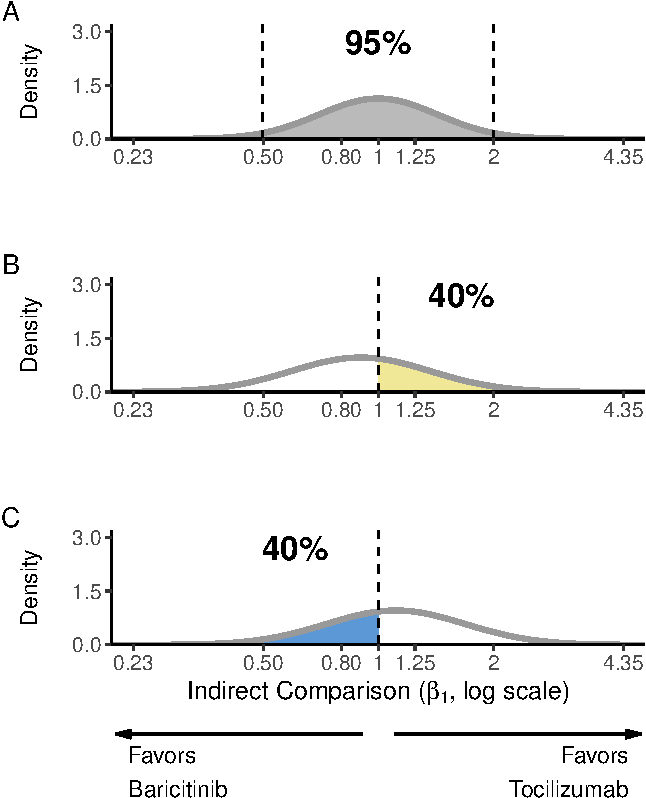
\includegraphics{supplementary_material_files/figure-latex/unnamed-chunk-2-1} \end{center}

Prior distributions for \(beta\_{1, Bari}\) (ratio of odds ratios) in
models comparing baricitinib to tocilizumab. Panel A: `Skeptical' prior.
The Normal(\(0\), \(0.354^2\)) distribution approximately concentrates
\(95\)\% of probability density between \(0.5\) and \(2.0\) in the
linear scale (\(-0.69\) and \(0.69\) in the log scale, respectively).
Panel B: `Optimistic for Baricitinib' prior. The Normal(\(-0.105\),
\(0.41^2\)) distribution approximately concentrates \(40\)\% of
probability density above \(1\). Panel C: `Optimistic for Tocilizumab'
prior. The Normal(\(0.105\), \(0.41^2\)) distribution approximately
concentrates \(40\)\% of probability density below \(1\).

\newpage

In summary, both sarilumab and baricitinib models can be fully described
as:

\begin{align*}
y_i & \sim Normal(\theta_i, \sigma_i^2)\\
\theta_i & \sim Normal(\mu, \tau^2)\\
\mu &= \beta_0 + \beta_{1, T} x_i\\
\end{align*}

while the priors in sarilumab's models are:

\begin{align*}
\beta_0 & \sim \operatorname{Normal}(0, 0.75^2)\\
\tau & \sim \operatorname{Log-Normal}(-1.975, 0.67^2)\\
\beta_{1, Sari[Skeptical]} & \sim \operatorname{Normal}(0, 0.354^2)\\
\beta_{1, Sari[Sarilumab]} & \sim \operatorname{Normal}(-0.049, 0.193^2)\\
\beta_{1, Sari[Tocilizumab]} & \sim \operatorname{Normal}(0.049, 0.193^2)\\
\beta_{1, Sari[Vague]} & \sim \operatorname{Normal}(0, 4^2)
\end{align*}

and the priors in baricitinib's models are:

\begin{align*}
\beta_0 & \sim \operatorname{Normal}(0, 0.75^2)\\
\tau & \sim \operatorname{Log-Normal}(-1.975, 0.67^2)\\
\beta_{1, Bari[Skeptical]} & \sim \operatorname{Normal}(0, 0.354^2)\\
\beta_{1, Bari[Baricitinib]} & \sim \operatorname{Normal}(-0.105, 0.416^2)\\
\beta_{1, Bari[Tocilizumab]} & \sim \operatorname{Normal}(0.105, 0.416^2)\\
\beta_{1, Bari[Vague]} & \sim \operatorname{Normal}(0, 4^2)
\end{align*}

where all parameters are in the log scale.

One could argue that baricitinib's priors are stronger than sarilumab's
given differences on the mean values (\(|0.105| > |0.049|\)). We note
that, although the mean values are different because we only found prior
evidence for the sarilumab vs.~tocilizumab comparison, these prior
discrepancies are likely to be of little relevance. As depicted in the
figures above, the baricitinib's priors have a greater mean but lower
density than sarilumab's priors. Therefore, we do not expect these
priors' impact on each marginal posterior distribution to be relevantly
different.

\newpage

\hypertarget{post-hoc-sensitivity-analysis}{%
\subsubsection{Post-hoc Sensitivity
Analysis}\label{post-hoc-sensitivity-analysis}}

Regarding the sarilumab vs.~tocilizumab meta-regression model, we also
performed a post-hoc sensitivity analysis with a different set of
priors.

We fitted the exact same model, but with different ``Optimistic for
Sarilumab'' and ``Optimistic for Tocilizumab'' priors (hereafter,
``Optimistic for Sarilumab (REMAP-CAP)'' and ``Optimistic for
Tocilizumab (inverse REMAP-CAP)'':

\begin{align*}
y_i & \sim Normal(\theta_i, \sigma_i^2) \tag{Likelihood}\\
\theta_i & \sim Normal(\mu, \tau^2)\\
\mu &= \beta_0 + \beta_{1, Sari} x_i\\
\\
\beta_0 & \sim \operatorname{Normal}(0, 0.75^2) \tag{Priors}\\
\tau & \sim \operatorname{Log-Normal}(-1.975, 0.67^2)\\
\beta_{1, Sari[Sarilumab]} & \sim \operatorname{Normal}(-0.049, 0.118^2)\\
\beta_{1, Sari[Tocilizumab]} & \sim \operatorname{Normal}(0.049, 0.118^2)\\
\end{align*}

These priors were constructed to reflect the exact same strength of the
single study that directly compared sarilumab to
tocilizumab.(\protect\hyperlink{ref-zotero-3144}{7})

The new standard deviation of \(0.118\) was obtained through the
formula:(\protect\hyperlink{ref-cochrane632}{12})

\[\sigma = \frac{\ln(\operatorname{UCL}) - \ln(\operatorname{LCL})}{3.92}\]

where \(UCL\) is \(1.35\), and \(LCL\) is \(0.85\), as depicted in the
Figure S3 of the RCT cited above (REMAP-CAP). In comparison to the 40\%
probability density above/below \(1.0\) yielded by the main priors in
the section before, these sensitivity priors yield \(34\%\),
highlighting its greater strength.

\newpage

\hypertarget{noninferiority-analysis}{%
\subsubsection{Noninferiority Analysis}\label{noninferiority-analysis}}

Our primary goal is to assess whether sarilumab and baricitinib are
noninferior to tocilizumab. Thus, we calculated the posterior
probabilities of noninferiority based on the marginal posterior
distributions of \(\beta_{1, T}\) in all models and scenarios described
above.

One major criteria in noninferiority analyses is that superiority of
active comparator --- in this case, tocilizumab --- in comparison to
control has been shown.(\protect\hyperlink{ref-tsui2019}{13}) The WHO
meta-analysis presented results in favor of tocilizumab's
superiority.(\protect\hyperlink{ref-whoma}{14}) Thus, we will use the
following formula to estimate our noninferiority
margin:(\protect\hyperlink{ref-trone2020}{15})

\begin{align*}
\gamma =  \left( \frac{1}{\theta} \right)^{1 - x} \\
\end{align*}

where \(\gamma\) is the estimated noninferiority margin, \(\theta\) is
the tocilizumab's mean effect size, and \(x\) is the percentage of
tocilizumab's effect that is desired to be preserved. Regarding
\(\theta\), we extracted the mean odds ratio regarding tocilizumab's
effect in the subgroup of patients using corticosteroids (page 14 in
their Supplement 2 (\protect\hyperlink{ref-whoma}{14})). We chose this
subgroup because it represents our population of interest. Moreover, we
will follow the U.S. Department of Health and Human Services Food and
Drug Administration's recommendation and define \(x\) as \(50\%\) for
our primary noninferiority
analysis.(\protect\hyperlink{ref-tsui2019}{13},\protect\hyperlink{ref-fda}{16})
Thus, our main noninferiority margin (in the linear scale) will be:

\begin{align*}
\gamma =  \left( \frac{1}{0.77} \right)^{0.5} = 1.139606 \\
\end{align*}

\newpage

\hypertarget{appendix-references}{%
\subsection{Appendix References}\label{appendix-references}}

\hypertarget{refs}{}
\begin{CSLReferences}{0}{0}
\leavevmode\vadjust pre{\hypertarget{ref-pedroza2018}{}}%
\CSLLeftMargin{1. }
\CSLRightInline{Pedroza C, Han W, Thanh Truong VT, Green C, Tyson JE.
Performance of informative priors skeptical of large treatment effects
in clinical trials: A simulation study. Stat Methods Med Res
{[}Internet{]}. 2018 Jan 1 {[}cited 2021 Sep 11{]};27(1):79--96.
Available from: \url{https://doi.org/10.1177/0962280215620828}}

\leavevmode\vadjust pre{\hypertarget{ref-turner2015}{}}%
\CSLLeftMargin{2. }
\CSLRightInline{Turner RM, Jackson D, Wei Y, Thompson SG, Higgins JPT.
Predictive distributions for between-study heterogeneity and simple
methods for their application in Bayesian meta-analysis. Statistics in
Medicine {[}Internet{]}. 2015 {[}cited 2021 May 8{]};34(6):984--98.
Available from:
\url{https://onlinelibrary.wiley.com/doi/abs/10.1002/sim.6381}}

\leavevmode\vadjust pre{\hypertarget{ref-spiegelhalter2004}{}}%
\CSLLeftMargin{3. }
\CSLRightInline{Spiegelhalter DJ, Abrams KR, Myles JP. Bayesian
approaches to clinical trials and health care evaluation. Chichester\,;
Hoboken, NJ: Wiley; 2004. 391 p. (Statistics in practice). }

\leavevmode\vadjust pre{\hypertarget{ref-rover2021}{}}%
\CSLLeftMargin{4. }
\CSLRightInline{Röver C, Bender R, Dias S, Schmid CH, Schmidli H, Sturtz
S, et al. On weakly informative prior distributions for the
heterogeneity parameter in Bayesian random-effects meta-analysis.
Research Synthesis Methods {[}Internet{]}. 2021 {[}cited 2021 Sep
2{]};12(4):448--74. Available from:
\url{https://onlinelibrary.wiley.com/doi/abs/10.1002/jrsm.1475}}

\leavevmode\vadjust pre{\hypertarget{ref-welton2020}{}}%
\CSLLeftMargin{5. }
\CSLRightInline{Welton NJ, Jones HE, Dias S. Bayesian Methods for
Meta-Analysis. In: Bayesian Methods in Pharmaceutical Research. Chapman
and Hall/CRC; 2020. }

\leavevmode\vadjust pre{\hypertarget{ref-higgins2009}{}}%
\CSLLeftMargin{6. }
\CSLRightInline{Higgins JPT, Thompson SG, Spiegelhalter DJ. A
re-evaluation of random-effects meta-analysis. Journal of the Royal
Statistical Society: Series A (Statistics in Society) {[}Internet{]}.
2009 {[}cited 2021 Jun 28{]};172(1):137--59. Available from:
\url{https://rss.onlinelibrary.wiley.com/doi/abs/10.1111/j.1467-985X.2008.00552.x}}

\leavevmode\vadjust pre{\hypertarget{ref-zotero-3144}{}}%
\CSLLeftMargin{7. }
\CSLRightInline{Effectiveness of Tocilizumab, Sarilumab, and Anakinra
for critically ill patients with COVID-19 The REMAP-CAP COVID-19 Immune
Modulation Therapy Domain Randomized Clinical Trial. :21. }

\leavevmode\vadjust pre{\hypertarget{ref-dias2018}{}}%
\CSLLeftMargin{8. }
\CSLRightInline{Dias S, editor. Network meta-analysis for decision
making. Hoboken, NJ: Wiley; 2018. 1 p. (Wiley Series in Statistics in
Practice). }

\leavevmode\vadjust pre{\hypertarget{ref-pitchforth2012}{}}%
\CSLLeftMargin{9. }
\CSLRightInline{Pitchforth JO, Mengersen KL. Bayesian Meta-Analysis. In:
Case Studies in Bayesian Statistical Modelling and Analysis
{[}Internet{]}. John Wiley \& Sons, Ltd; 2012 {[}cited 2022 Mar 5{]}. p.
118--40. Available from:
\url{https://onlinelibrary.wiley.com/doi/abs/10.1002/9781118394472.ch7}}

\leavevmode\vadjust pre{\hypertarget{ref-thompson2002}{}}%
\CSLLeftMargin{10. }
\CSLRightInline{Thompson SG, Higgins JPT. How should meta-regression
analyses be undertaken and interpreted? Statist Med {[}Internet{]}. 2002
Jun 15 {[}cited 2021 Sep 7{]};21(11):1559--73. Available from:
\url{https://onlinelibrary.wiley.com/doi/10.1002/sim.1187}}

\leavevmode\vadjust pre{\hypertarget{ref-zampieri2021}{}}%
\CSLLeftMargin{11. }
\CSLRightInline{Zampieri FG, Casey JD, Shankar-Hari M, Harrell FE,
Harhay MO. Using Bayesian Methods to Augment the Interpretation of
Critical Care Trials. An Overview of Theory and Example Reanalysis of
the Alveolar Recruitment for Acute Respiratory Distress Syndrome Trial.
Am J Respir Crit Care Med {[}Internet{]}. 2021 Mar 1 {[}cited 2021 Mar
1{]};203(5):543--52. Available from:
\url{https://www.atsjournals.org/doi/10.1164/rccm.202006-2381CP}}

\leavevmode\vadjust pre{\hypertarget{ref-cochrane632}{}}%
\CSLLeftMargin{12. }
\CSLRightInline{Higgins J, Thomas J, Chandler J, Cumpston M, Li T, Page
M, et al., editors. Cochrane Handbook for Systematic Reviews of
Interventions version 6.2 (updated February 2021) {[}Internet{]}.
Cochrane; 2021 {[}cited 2022 Jan 15{]}. Available from:
\url{https://training.cochrane.org/handbook}}

\leavevmode\vadjust pre{\hypertarget{ref-tsui2019}{}}%
\CSLLeftMargin{13. }
\CSLRightInline{Tsui M, Rehal S, Jairath V, Kahan BC. Most
noninferiority trials were not designed to preserve active comparator
treatment effects. Journal of Clinical Epidemiology {[}Internet{]}. 2019
Jun 1 {[}cited 2022 Mar 5{]};110:82--9. Available from:
\url{https://www.jclinepi.com/article/S0895-4356(18)30599-7/fulltext}}

\leavevmode\vadjust pre{\hypertarget{ref-whoma}{}}%
\CSLLeftMargin{14. }
\CSLRightInline{The WHO Rapid Evidence Appraisal for COVID-19 Therapies
(REACT) Working Group. Association Between Administration of IL-6
Antagonists and Mortality Among Patients Hospitalized for COVID-19: A
Meta-analysis. JAMA {[}Internet{]}. 2021 Aug 10 {[}cited 2021 Sep
2{]};326(6):499--518. Available from:
\url{https://doi.org/10.1001/jama.2021.11330}}

\leavevmode\vadjust pre{\hypertarget{ref-trone2020}{}}%
\CSLLeftMargin{15. }
\CSLRightInline{Trone J-C, Ollier E, Chapelle C, Mismetti P, Cucherat M,
Magné N, et al. Assessment of non-inferiority with meta-analysis:
example of hypofractionated radiation therapy in breast and prostate
cancer. Sci Rep {[}Internet{]}. 2020 Sep 22 {[}cited 2022 Mar
5{]};10(1):15415. Available from:
\url{https://www.nature.com/articles/s41598-020-72088-2}}

\leavevmode\vadjust pre{\hypertarget{ref-fda}{}}%
\CSLLeftMargin{16. }
\CSLRightInline{U.S. Department of Health and Human Services Food and
Drug Administration. Non-Inferiority Clinical Trials to Establish
Effectiveness Guidance for Industry {[}Internet{]}. 2016. Available
from: \url{https://www.fda.gov/media/78504/download}}

\end{CSLReferences}

\begin{landscape}

\hypertarget{appendix-results}{%
\section{Appendix Results}\label{appendix-results}}

\hypertarget{appendix-figure-1-prisma-2020-flow-diagram}{%
\subsection{Appendix Figure 1: PRISMA 2020 Flow
Diagram}\label{appendix-figure-1-prisma-2020-flow-diagram}}

\begin{center}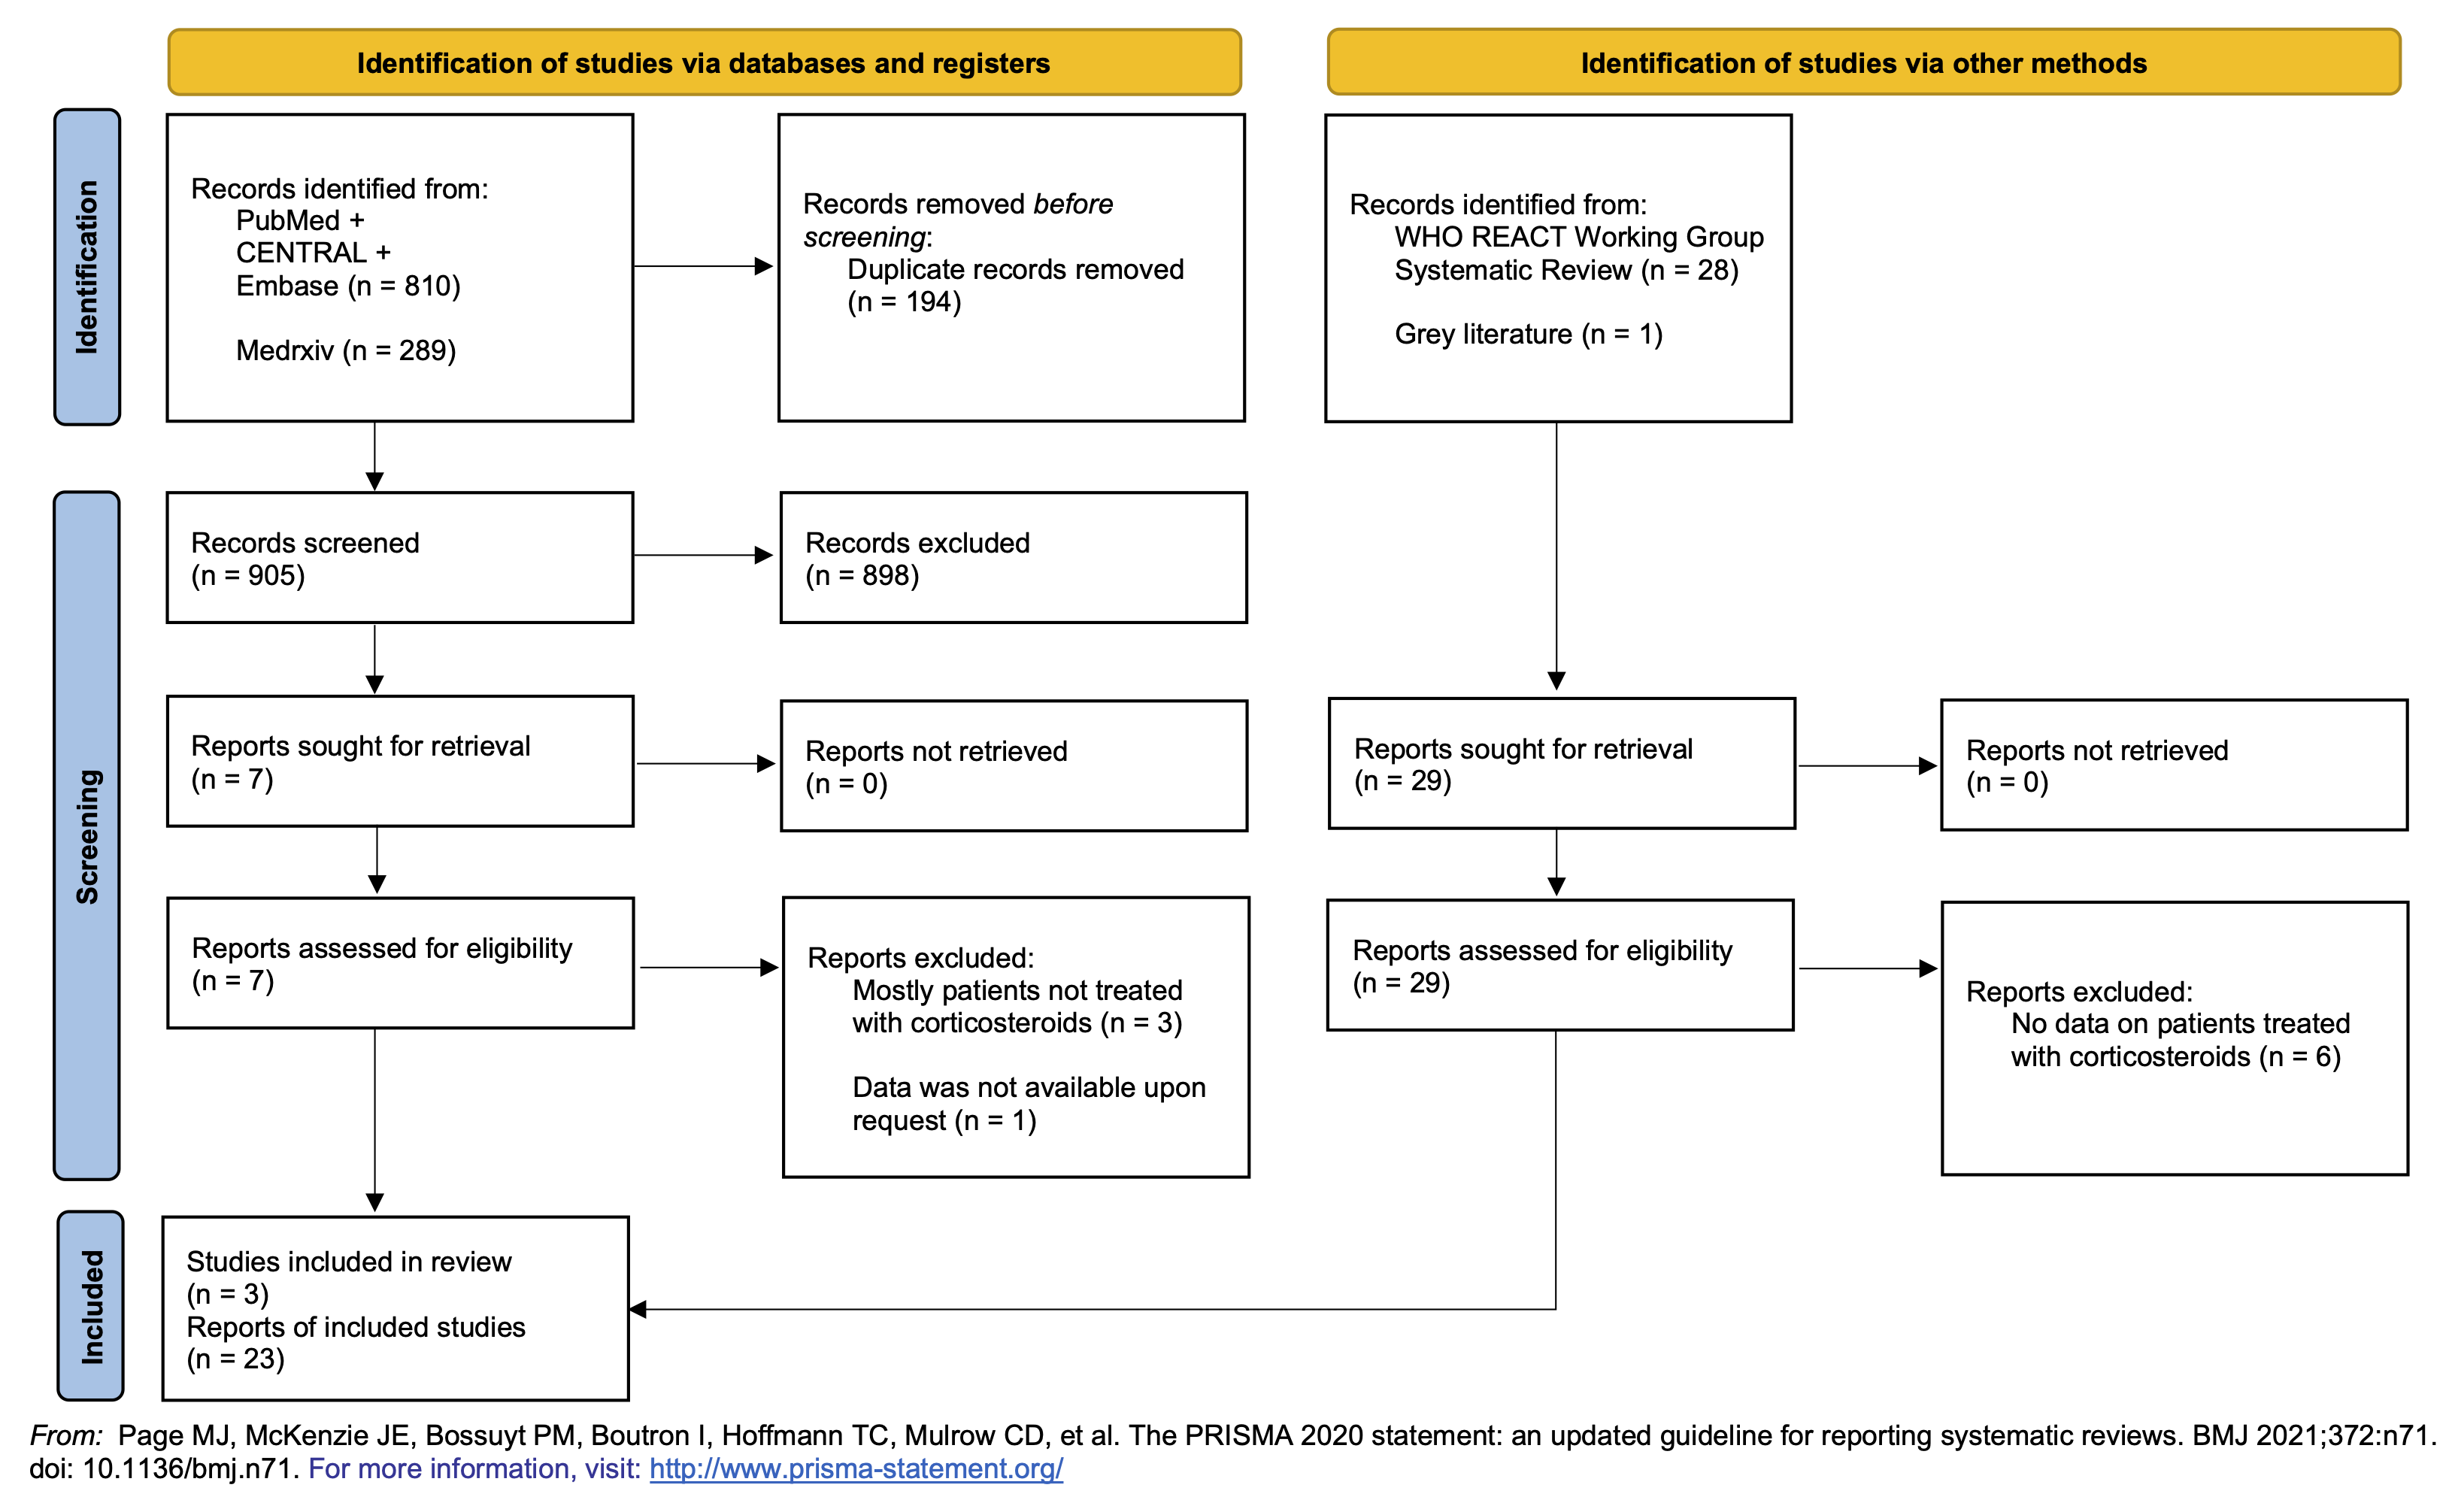
\includegraphics[width=0.88\linewidth]{/Users/arthur/Coding/projects/active/toci_sari_bari/PRISMA_2020_flow_diagram_correct} \end{center}

\end{landscape}

\hypertarget{appendix-figure-2-risk-of-bias-assessment}{%
\subsection{Appendix Figure 2: Risk of Bias
Assessment}\label{appendix-figure-2-risk-of-bias-assessment}}

\begin{center}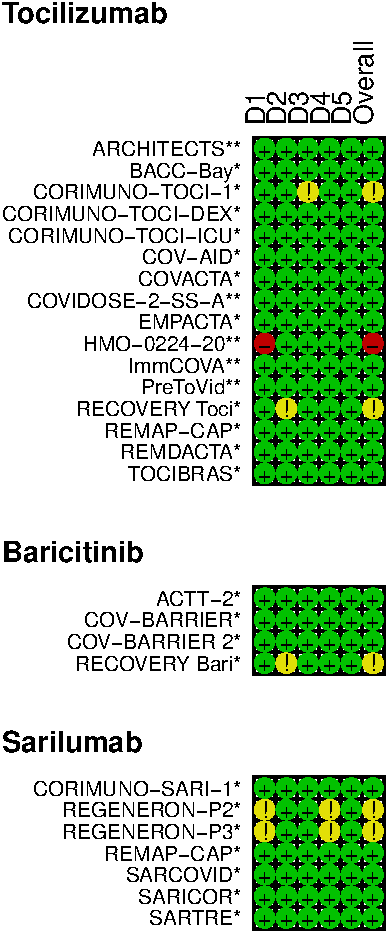
\includegraphics{supplementary_material_files/figure-latex/unnamed-chunk-5-1} \end{center}

Risk of bias for domain-level as well as overall judgement for each
individual study.

D1: bias arising from randomisation process; D2: bias arising from
deviations from intended interventions; D3: bias due to missing outcome
data; D4: bias in measurement of the outcome; D5: bias in selection of
the reported result.

``+'' depicts ``Low'' risk, while ``!'' and ``-'' indicate ``Some
concerns'' and ``High,'' respectively.

Studies with * indicate that the risk of bias assessment was performed
by our research group. In contrast, ** indicates that the assessment was
performed by the WHO React Working Group, as explained in our Methods
section.

\hypertarget{appendix-figure-3-risk-of-bias-proportion}{%
\subsection{Appendix Figure 3: Risk of Bias
Proportion}\label{appendix-figure-3-risk-of-bias-proportion}}

\begin{center}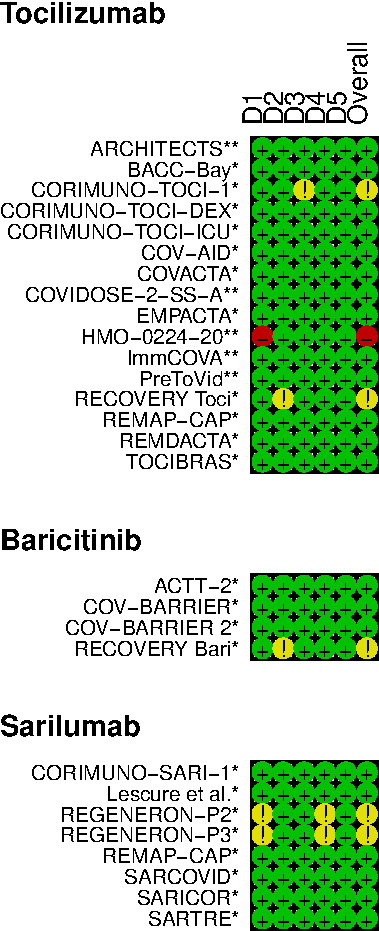
\includegraphics{supplementary_material_files/figure-latex/unnamed-chunk-6-1} \end{center}

Distributions of proportions of risk of bias within each domain. Panel
A: Tocilizumab studies; Panel B: Baricitinib; Panel C: Sarilumab.

\newpage

\hypertarget{appendix-figure-4-posterior-probabilities-odds-ratio}{%
\subsection{Appendix Figure 4: Posterior Probabilities (Odds
Ratio)}\label{appendix-figure-4-posterior-probabilities-odds-ratio}}

\begin{center}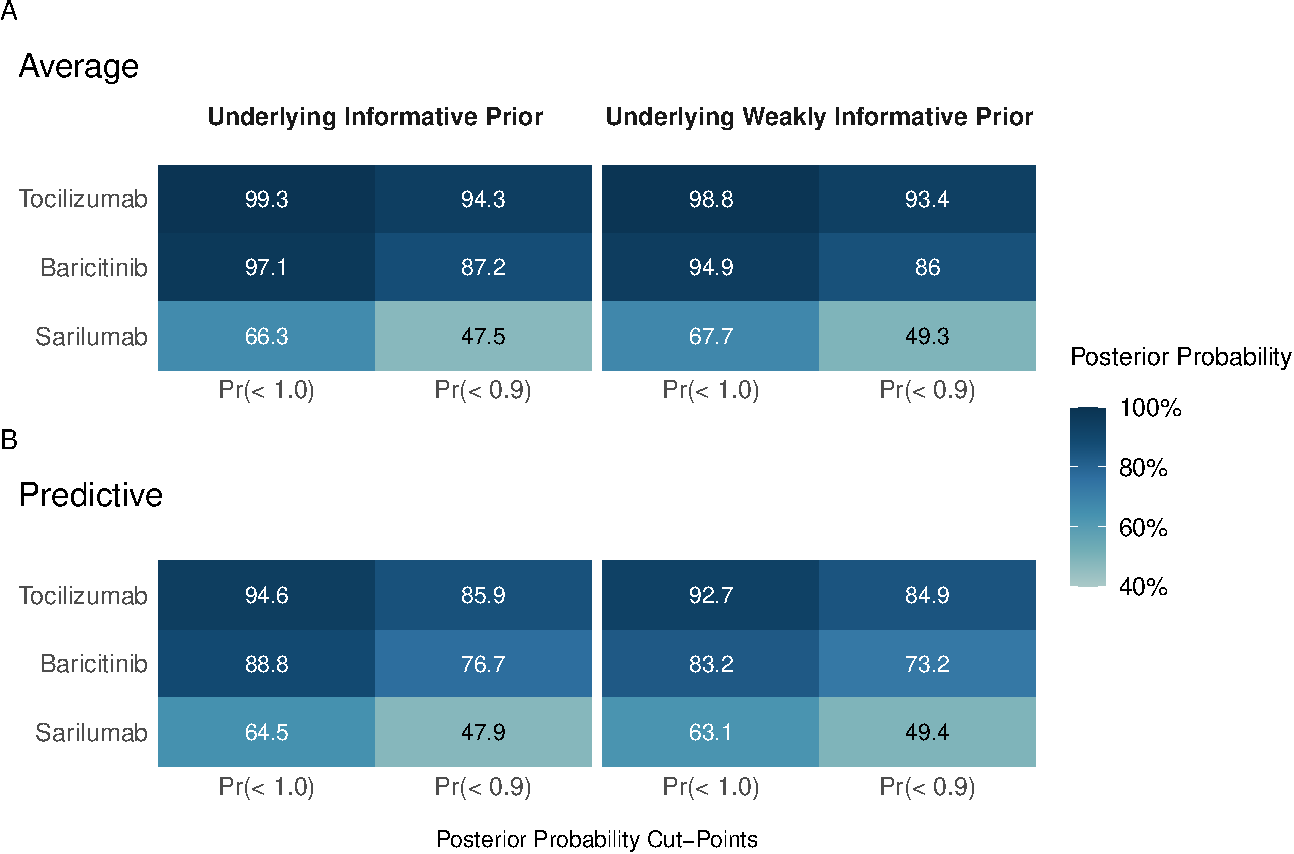
\includegraphics{supplementary_material_files/figure-latex/posterior probabilities heatmap-1} \end{center}

Heatmaps with posterior probabilities of tocilizumab, baricitinib, and
sarilumab meta-analyses' average (Panel A) and predictive effect (Panel
B). \emph{``Pr(\textless{} 1.0)''} depicts probabilities of any benefit
(\textless{} 1.0 odds ratio {[}OR{]}), and \emph{``Pr(\textless{}
0.9)''} depicts probabilities of clinically meaningful benefit
(\textless{} 0.9 OR). The exact probability is shown in each cell, while
darker colors correspond to higher probabilities.

Heatmaps on the left regard models assuming a more informative prior
(\(\operatorname{Log-Normal}[-1.975, 0.67^2]\)) for the between-study
standard deviation, while heatmaps on the right regard models with
weakly informative prior (\(\operatorname{Half-Normal}[0.5^2]\)). All
models assume a \(Normal(0, 0.75^2)\) prior distribution for average
effect (\(\mu\)).

\newpage

\hypertarget{appendix-figure-5-baricitinib-sensitivity-meta-analysis}{%
\subsection{Appendix Figure 5: Baricitinib Sensitivity
Meta-Analysis}\label{appendix-figure-5-baricitinib-sensitivity-meta-analysis}}

\begin{center}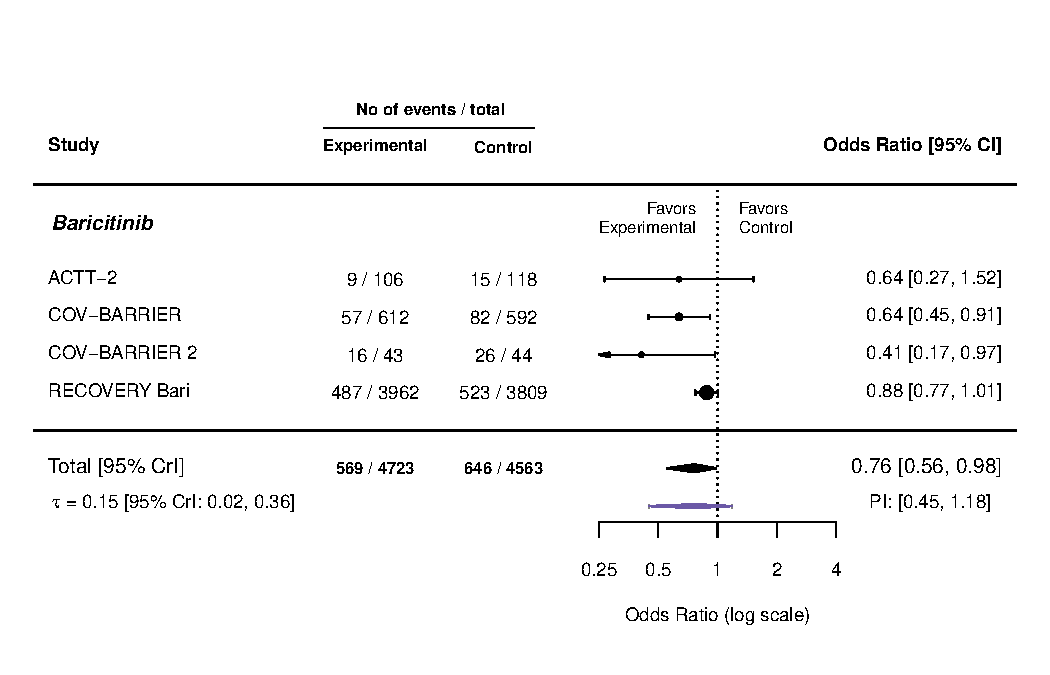
\includegraphics[width=29.17in]{/Users/arthur/Coding/projects/active/toci_sari_bari/output/figures/supplementary/forest_sari_sens} \end{center}

Sensitivity analysis including all patients treated with
corticosteroids, regardless of tocilizumab use, in RECOVERY Bari.

Forest plot of Bayesian random-effect meta-analysis of baricitinib
versus control. Black diamond represents the median and 95\% credible
interval of posterior overall effect (\(\mu\)). Purple diamonds
represents the 95\% prediction interval on the posterior predictive
distribution. The median and 95\% credible interval of the between-study
standard deviation parameter (\(\tau\)) are displayed on the left bottom
corner. Abbreviations: RE, random-effect; CrI, credible interval; PI,
prediction interval.

\newpage

\hypertarget{appendix-figure-6-posterior-distributions-risk-difference}{%
\subsection{Appendix Figure 6: Posterior Distributions (Risk
Difference)}\label{appendix-figure-6-posterior-distributions-risk-difference}}

\begin{center}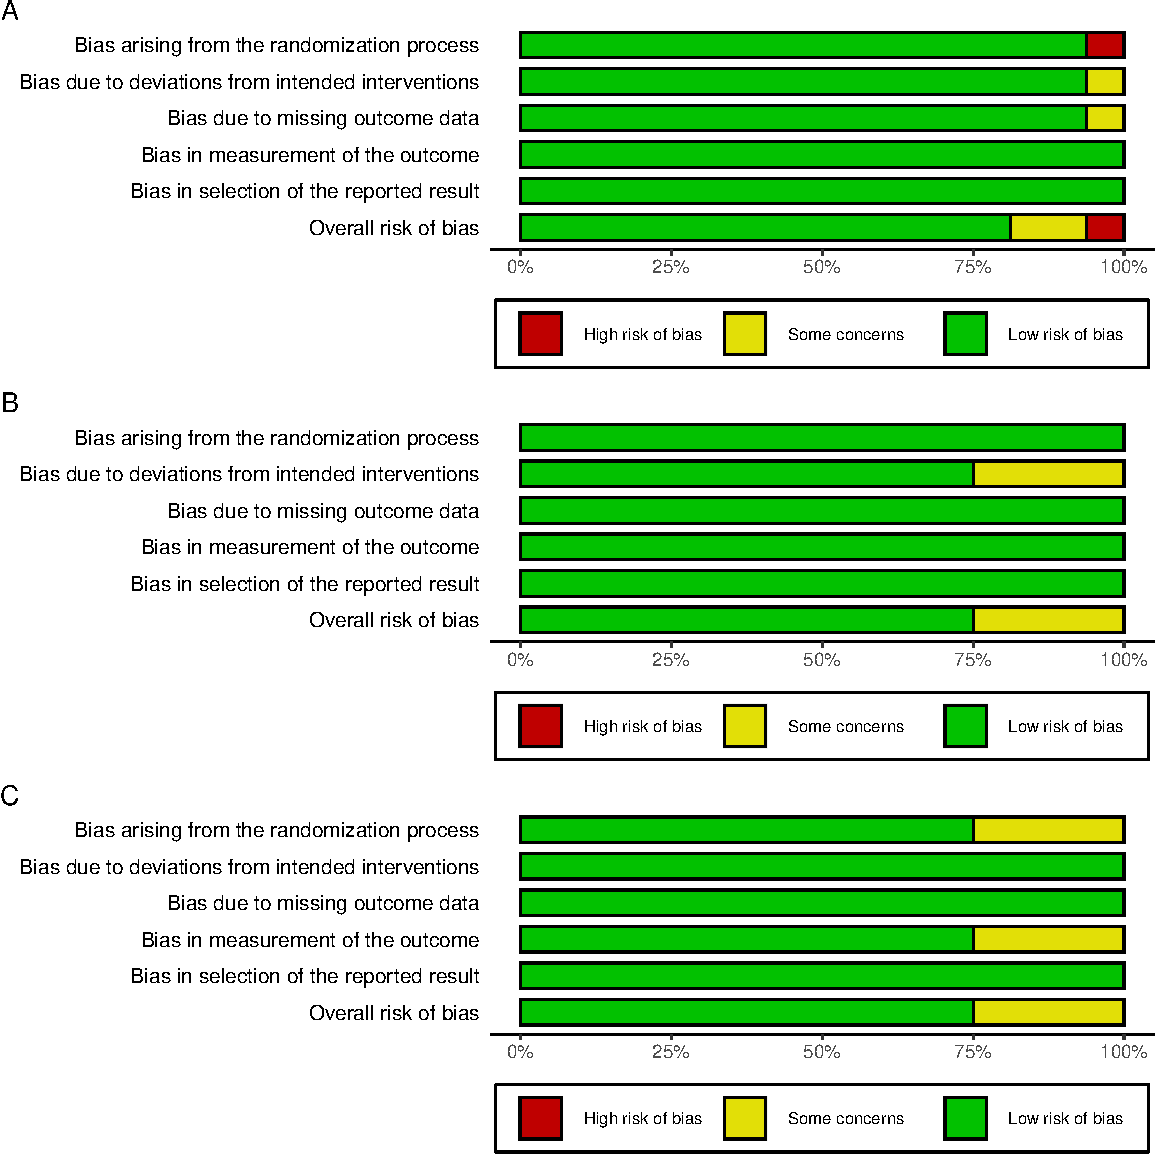
\includegraphics{supplementary_material_files/figure-latex/unnamed-chunk-8-1} \end{center}

Meta-analysis average effect marginal posterior distributions in the
risk difference scale (Y-axis) across multiple mortality risks under
control treatment (X-axis) for each experimental drug. Black solid lines
represent the median, darker colored areas represent the 95\% CrIs of
average effect, and lighter areas represent the 95\% CrIs of predictive
effect. Risk difference greater than 0 favors experimental drug over
control.

Underlying prior distributions are \(Normal(0, 0.75^2)\) for the average
effect (\(\mu\)), and \(\operatorname{Log-Normal}[-1.975, 0.67^2]\) for
the between-study standard deviation (\(\tau\)).

Abbreviation: CrI, credible interval

\newpage

\hypertarget{appendix-figure-7-posterior-probabilities-risk-difference}{%
\subsection{Appendix Figure 7: Posterior Probabilities (Risk
Difference)}\label{appendix-figure-7-posterior-probabilities-risk-difference}}

\begin{center}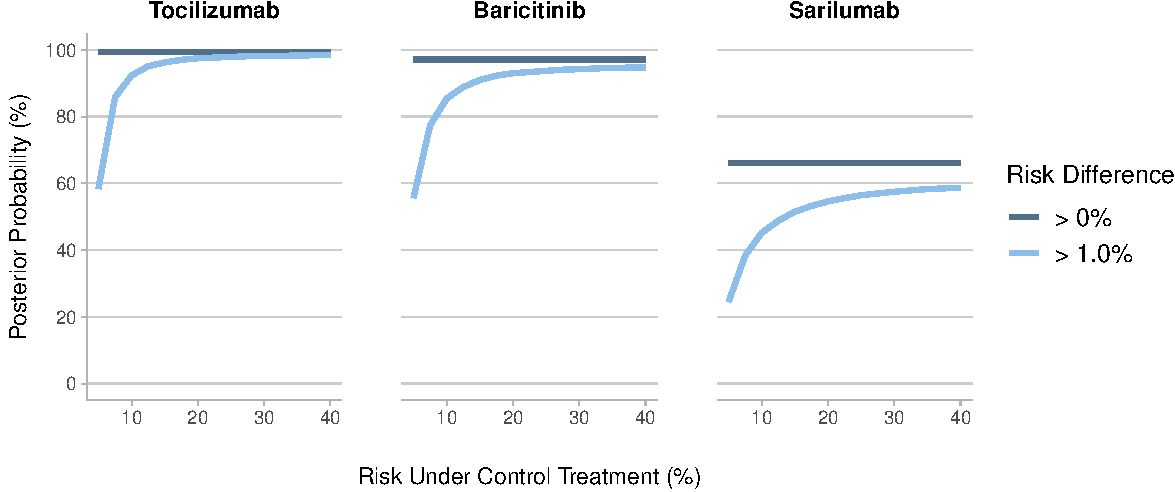
\includegraphics{supplementary_material_files/figure-latex/RD probabilities plot-1} \end{center}

Average effect posterior probabilities of benefit in the risk difference
scale. Each line represents the posterior probability for a specific
cut-point, such as risk difference greater than 0\% or 1\%. across
multiple mortality risks under control treatment.

Underlying prior distributions are \(Normal(0, 0.75^2)\) for the average
effect (\(\mu\)), and \(\operatorname{Log-Normal}[-1.975, 0.67^2]\) for
the between-study standard deviation (\(\tau\)).

\newpage

\hypertarget{appendix-figure-8-posterior-between-study-standard-deviations}{%
\subsection{Appendix Figure 8: Posterior Between-Study Standard
Deviations}\label{appendix-figure-8-posterior-between-study-standard-deviations}}

\begin{center}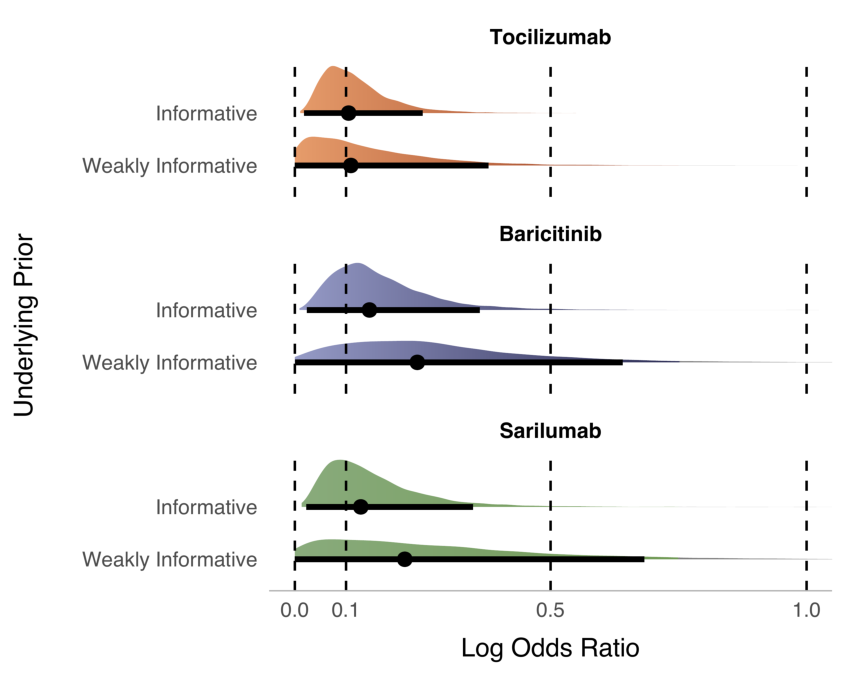
\includegraphics{supplementary_material_files/figure-latex/tau figure display-1} \end{center}

Between study standard deviation (\(\tau\)) marginal posterior
distributions upon different underlying prior distributions (informative
or weakly informative) for \(\tau\). This parameter is an estimate for
between-study heterogeneity in random-effect meta-analyses. Point
estimates depict the median, while intervals bars 95\% CrIs. Dashed
lines represent different heterogeneity ranges: from 0 to 0.1 log odds
ratio, ``Low heterogeneity''; from 0.1 to 0.5, ``Reasonable''; from 0.5
to 1.0, ``Fairly High'' (per Spiegelhalter et al.,
(\protect\hyperlink{ref-spiegelhalter2004}{3})).

For \(\tau\), the ``Informative'' prior regards a
\(\operatorname{Log-Normal}(-1.975, 0.67^2)\) distribution, while
``Weakly Informative'' regards a \(\operatorname{Half-Normal}(0.5)\)
distribution. All models assume a \(Normal(0, 0.75^2)\) prior
distribution for average effect (\(mu\)).

Abbreviation: CrI, credible interval

\newpage

\hypertarget{appendix-table-1-posterior-probabilities-of-heterogeneity} \\ 
 \cmidrule(lr){2-4}
 & Low & Reasonable & Fairly High \\ 
\midrule
\multicolumn{1}{l}{Tocilizumab} \\ 
\midrule
Informative & 46.3 & 53.6 & 0.0 \\ 
Weakly Informative & 46.2 & 52.1 & 1.6 \\ 
\midrule
\multicolumn{1}{l}{Baricitinib} \\ 
\midrule
Informative & 20.6 & 77.9 & 1.5 \\ 
Weakly Informative & 11.2 & 73.6 & 14.5 \\ 
\midrule
\multicolumn{1}{l}{Sarilumab} \\ 
\midrule
Informative & 34.5 & 64.5 & 1.0 \\ 
Weakly Informative & 24.6 & 61.7 & 13.2 \\ 
 \bottomrule
\end{longtable}
\begin{minipage}{\linewidth}
Low heterogeneity range: between 0 and 0.1 log odds ratio; Reasonable range: between 0.1 and 0.5; Fairly high: between 0.5 and 1.0.\\ 
\end{minipage}

\newpage

\hypertarget{appendix-table-2-meta-analyses-summary-results}{%
\subsection{Appendix Table 2: Meta-Analyses Summary
Results}\label{appendix-table-2-meta-analyses-summary-results}}

\captionsetup[table]{labelformat=empty,skip=1pt}
\begin{longtable}{lrrr}
\toprule
 & \multicolumn{3}{c}{Posterior Results, Median and 95\% CrI} \\ 
 \cmidrule(lr){2-4}
Treatment / Prior & Average Effect\textsuperscript{1} & Between-study SD\textsuperscript{2} & Predictive Effect\textsuperscript{1} \\ 
\midrule
\multicolumn{1}{l}{Tocilizumab} \\ 
\midrule
Informative & 0.78 [0.65, 0.94] & 0.11 [0.02, 0.25] & 0.78 [0.56, 1.1] \\ 
Weakly Informative & 0.78 [0.63, 0.97] & 0.11 [0, 0.38] & 0.78 [0.51, 1.24] \\ 
\midrule
\multicolumn{1}{l}{Baricitinib} \\ 
\midrule
Informative & 0.78 [0.56, 1.03] & 0.16 [0.03, 0.38] & 0.78 [0.44, 1.26] \\ 
Weakly Informative & 0.75 [0.46, 1.07] & 0.27 [0, 0.69] & 0.76 [0.31, 1.79] \\ 
\midrule
\multicolumn{1}{l}{Sarilumab} \\ 
\midrule
Informative & 0.92 [0.6, 1.41] & 0.13 [0.02, 0.35] & 0.92 [0.52, 1.62] \\ 
Weakly Informative & 0.91 [0.57, 1.51] & 0.21 [0, 0.68] & 0.92 [0.4, 2.21] \\ 
 \bottomrule
\end{longtable}
\vspace{-5mm}
\begin{minipage}{\linewidth}
\textsuperscript{1}Odds Ratio \\ 
\textsuperscript{2}Log Odds Ratio \\ 
\end{minipage}
\begin{minipage}{\linewidth}
Informative Between-study SD Prior: LN(-1.975, 0.67); Weakly Informative Prior: HN(0.5); LN(mu, SD) = Log-Normal(mean, SD); HN(SD) = Half-Normal(SD)\\ 
\end{minipage}

\newpage

\hypertarget{appendix-figure-9-funnel-plots}{%
\subsection{Appendix Figure 9: Funnel
Plots}\label{appendix-figure-9-funnel-plots}}

\begin{center}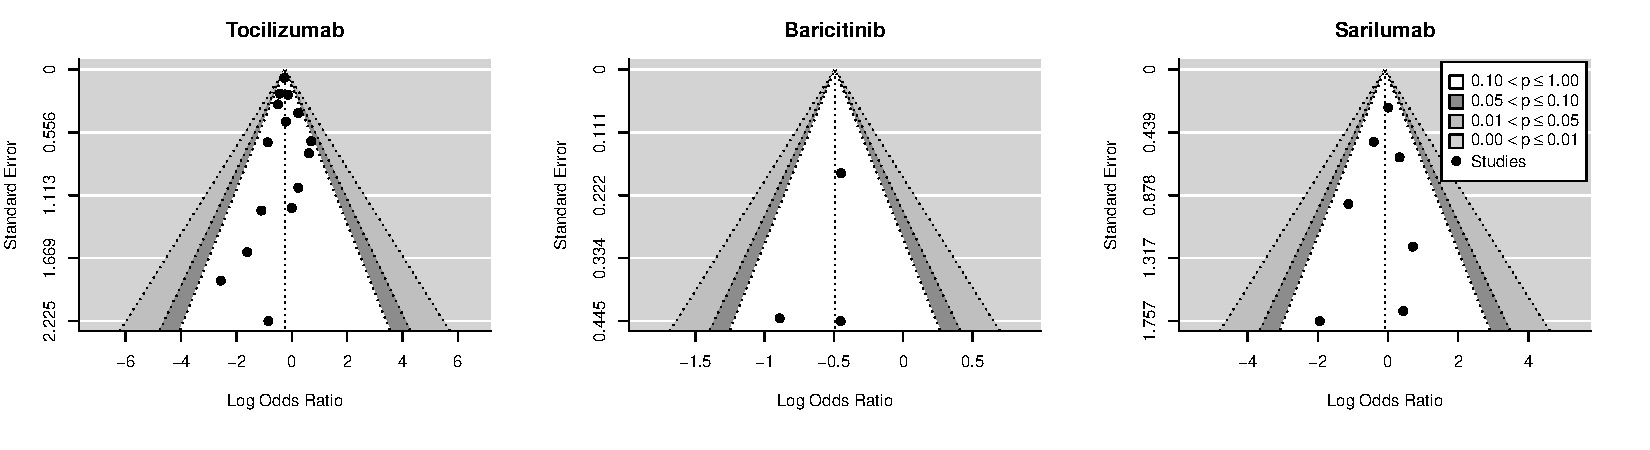
\includegraphics[width=15.39in,height=1.2\linewidth]{/Users/arthur/Coding/projects/active/toci_sari_bari/output/figures/supplementary/funnels} \end{center}

Contour-enhanced funnel plots for small study effect assessment.

\newpage

\newgeometry{left=0.5in,right=0.1in,top=0.5in,bottom=0.5in, noheadfoot}

\begin{landscape}

\hypertarget{appendix-table-3-certainty-of-evidence-grade}{%
\subsection{Appendix Table 3: Certainty of Evidence
(GRADE)}\label{appendix-table-3-certainty-of-evidence-grade}}

\begingroup\fontsize{10}{12}\selectfont

\begin{tabu} to \linewidth {>{\raggedright}X>{\raggedright}X>{\raggedright}X>{\raggedright}X>{\raggedright}X>{\raggedright}X>{\raggedright}X}
\hline
Drug & Risk of Bias & Heterogeneity & Imprecision & Indirectness & Publication Bias & Judgment\\
\hline
\cellcolor{gray!6}{Tocilizumab} & \cellcolor{gray!6}{We did not downgrade as the most weighted studies were judged as low risk of bias.} & \cellcolor{gray!6}{Certainty was downgraded by 2 levels due to serious heterogeneity as the prediction interval suggests future studies could estimate different results leading to opposite clinical decisions (upper bound of the confidence interval estimated as OR = 1.10) and substantial variability in point estimates across studies, both in magnitude and direction of effect.} & \cellcolor{gray!6}{We did not downgrade due to imprecision, although by a close call, despite reasonably large confidence intervals (35\% reduction to 6\% reduction in mortality) as the upper bound of the CI suggests clinically relevant benefit.} & \cellcolor{gray!6}{We did not find compelling evidence to downgrade due to indirectness.} & \cellcolor{gray!6}{We did not find compelling evidence to downgrade due to publication bias.} & \cellcolor{gray!6}{LOW QUALITY OF EVIDENCE, downgraded by 2 levels due to serious heterogeneity}\\
\hline
Baricitinib & We did not downgrade as the study contributing the most to the final result (COV-BARRIER), out of 3 studies, was judged as low risk of bias. & We did not downgrade, although by a close call, based on heterogeneity alone: point estimates are reasonably similar; heterogeneity as evidenced by tau is reasonable; the impact of the heterogeneity, as measured by the prediction interval, is that future studies may suggest an arguably irrelevant benefit in practice (1\% relative reduction in mortality) but does not include a null effect. & We did not downgrade, although by a close call, based on imprecision alone: clinical decision would likely not differ from worst-case (OR = 0.89) to best case (OR = 0.42) scenarios within the confidence interval; however, the final result is based on low total number of studies and outcome events leading to a large confidence interval. & We did not find compelling evidence to downgrade due to indirectness. & We did not find compelling evidence to downgrade due to publication bias. & MODERATE QUALITY OF EVIDENCE, downgraded 1 level due to imprecision and heterogeneity (two close calls)\\
\hline
\end{tabu}
\endgroup{}

\end{landscape}

\begin{landscape}

\begingroup\fontsize{10}{12}\selectfont

\begin{tabu} to \linewidth {>{\raggedright}X>{\raggedright}X>{\raggedright}X>{\raggedright}X>{\raggedright}X>{\raggedright}X>{\raggedright}X}
\hline
Drug & Risk of Bias & Heterogeneity & Imprecision & Indirectness & Publication Bias & Judgment\\
\hline
\cellcolor{gray!6}{Sarilumab} & \cellcolor{gray!6}{We did not downgrade as the most weighted studies were judged as low risk of bias.} & \cellcolor{gray!6}{Certainty was downgraded by 1 level due to substantial variability in point estimates, both in magnitude and direction of effect.} & \cellcolor{gray!6}{Certainty was downgraded by 2 levels due to serious imprecision (the confidence interval includes both clinically relevant benefits and harms).} & \cellcolor{gray!6}{We did not find compelling evidence to downgrade due to indirectness.} & \cellcolor{gray!6}{We did not find compelling evidence to downgrade due to publication bias.} & \cellcolor{gray!6}{VERY LOW QUALITY OF EVIDENCE, downgraded by 1 level due to heterogeneity and 2 levels due to serious imprecision.}\\
\hline
\end{tabu}
\endgroup{}

\end{landscape}

\restoregeometry

\newpage

\hypertarget{appendix-figure-9-sarilumab-vs.-tocilizumab-sensitivity-analysis}{%
\subsection{Appendix Figure 9: Sarilumab vs.~Tocilizumab Sensitivity
Analysis}\label{appendix-figure-9-sarilumab-vs.-tocilizumab-sensitivity-analysis}}

\begin{center}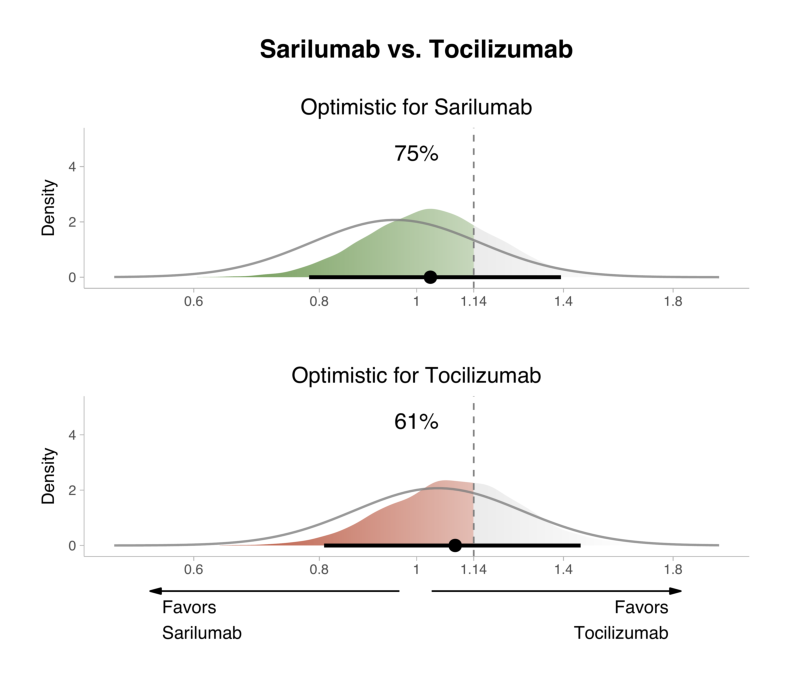
\includegraphics{supplementary_material_files/figure-latex/meta regressions sensitivity plot display-1} \end{center}

Post-hoc sensitivity analysis on sarilumab vs.~tocilizumab
meta-regression model (ratio of odds ratios). Color filled curves
represent marginal posterior distributions. Color filled areas represent
the posterior probability of noninferiority (Pr \textless{} 1.14), as
the percentages on top of each panel. Lastly, interval bars depict the
posterior median and 95\% credible intervals.

REMAP-CAP is an RCT that directly compared sarilumab to tocilizumab and
found results favoring sarilumab. We therefore created a prior
distribution to incorporate these results (``Optimistic for Sarilumab
(REMAP-CAP'')), and its inverse (``Optimistic for Tocilizumab (inverse
REMAP-CAP'')), as further explained in the Appendix Methods.

\newpage

\hypertarget{appendix-table-4-sarilumab-vs.-tocilizumab-sensitivity-analysis}{%
\subsection{Appendix Table 4: Sarilumab vs.~Tocilizumab Sensitivity
Analysis}\label{appendix-table-4-sarilumab-vs.-tocilizumab-sensitivity-analysis}}

\begin{tabu} to \linewidth {>{\raggedright}X>{\raggedright}X>{\raggedleft}X>{\raggedleft}X}
\toprule
Belief & ROR (95\% CrI) & Probability of Noninferiority, \% (1) & Probability of Superiority, \% (2)\\
\midrule
Optimistic for Sarilumab  (REMAP-CAP) & 0.99 (0.8, 1.21) & 90 & 52\\
 
Optimistic for Tocilizumab  (inverse REMAP-CAP) & 1.07 (0.88, 1.31) & 71 & 25\\
\bottomrule
\multicolumn{4}{l}{\rule{0pt}{1em}\textit{Note: }}\\
\multicolumn{4}{l}{\rule{0pt}{1em}Abbreviations: ROR, ratio of odds ratios; CrI, credibility interval}\\
\multicolumn{4}{l}{\rule{0pt}{1em}\textsuperscript{1} Probability of Noninferiority, \%}\\
\multicolumn{4}{l}{\rule{0pt}{1em}\textsuperscript{2} Probability of Superiority, \%}\\
\end{tabu}

\newpage

\hypertarget{appendix-figure-10-noninferiority-margin-sensitivity-analysis}{%
\subsection{Appendix Figure 10: Noninferiority Margin Sensitivity
Analysis}\label{appendix-figure-10-noninferiority-margin-sensitivity-analysis}}

\begin{center}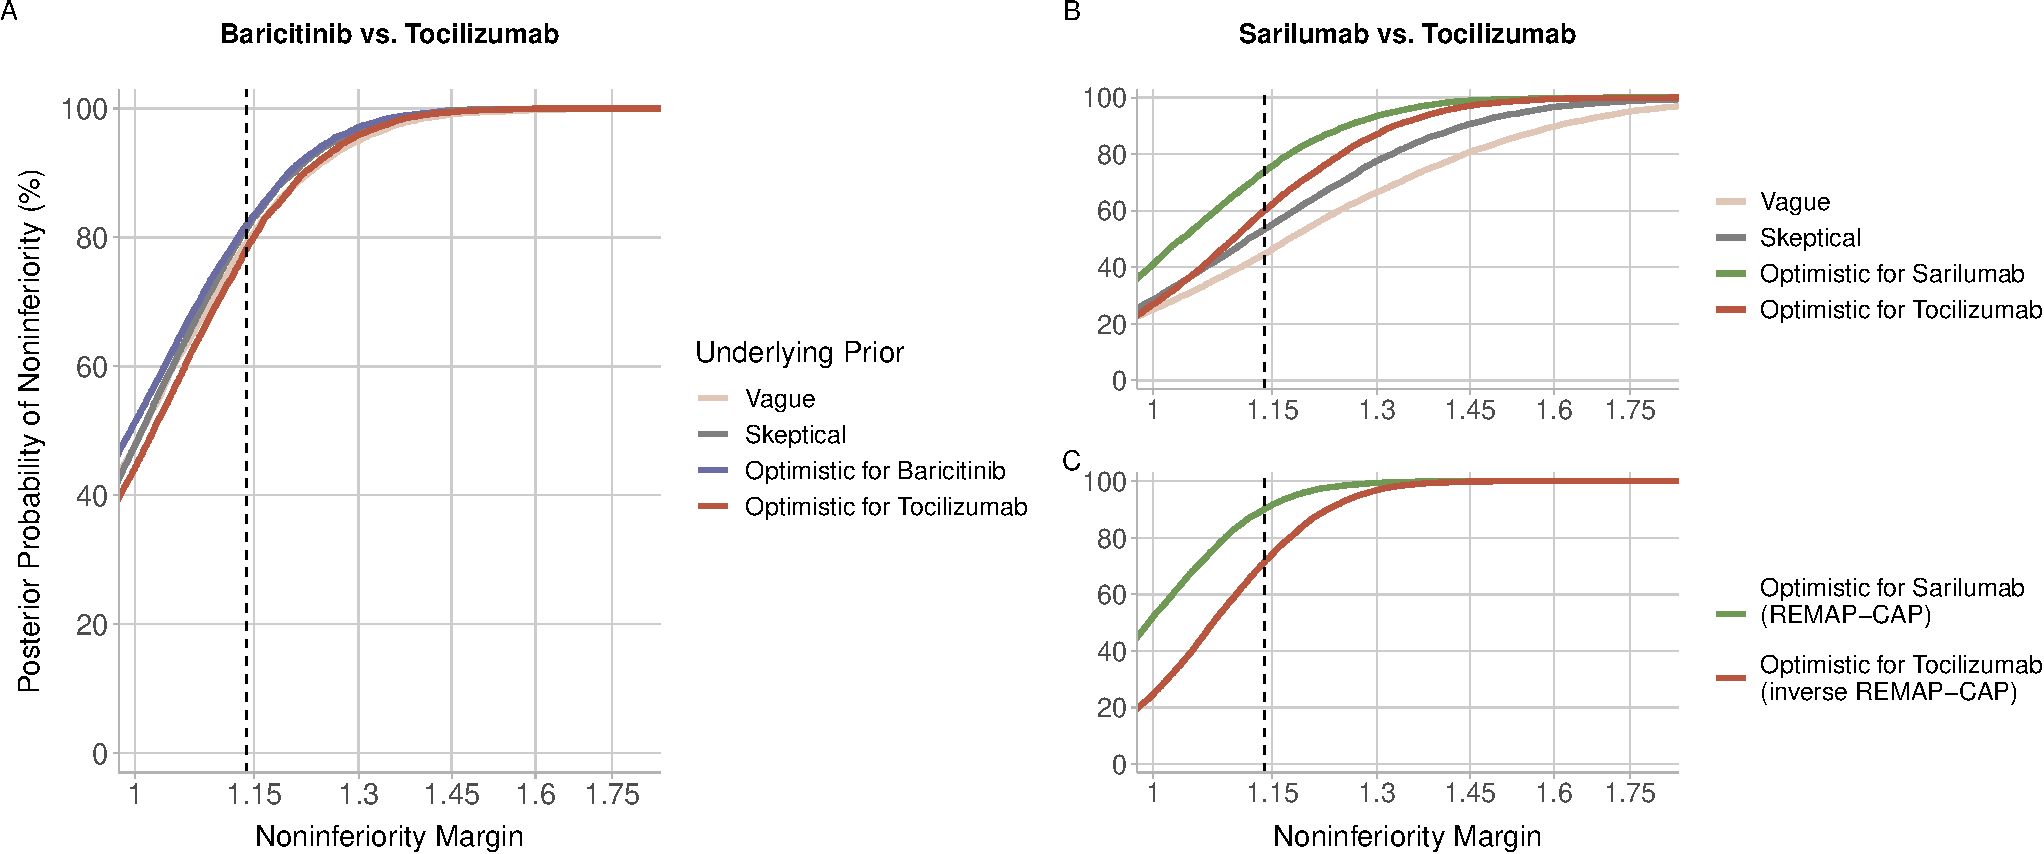
\includegraphics{supplementary_material_files/figure-latex/probabilities of noninferiority figure-1} \end{center}

Posterior probabilities (Y-axis) across multiple noninferiority margins
(X-axis) of meta-regressions models. Each curve represents a different
analysis based on the underlying prior distribution. The dashed black
line represents the main noninferiority margin (1.14 ratio of odds
ratios). Panel A depicts results regarding baricitinib vs.~tocilizumab
analyses. There is a zoomed-in panel to better represent differences
shown between 1.0 and 1.28 margins on the X-axis, and between 90 and
100\% on the Y-axis. Panel B depicts results regarding sarilumab
vs.~tocilizumab main analyses. Panel C depicts results regarding
sarilumab vs.~tocilizumab post-hoc sensitivity analyses.

\newpage

\hypertarget{appendix-table-5-baricitinib-vs.-tocilizumab-sensitivity-analysis}{%
\subsection{Appendix Table 5: Baricitinib vs.~Tocilizumab Sensitivity
Analysis}\label{appendix-table-5-baricitinib-vs.-tocilizumab-sensitivity-analysis}}

\begin{tabu} to \linewidth {>{\raggedright}X>{\raggedright}X>{\raggedleft}X>{\raggedleft}X}
\toprule
Belief & ROR (95\% CrI) & Probability of Noninferiority, \% (1) & Probability of Superiority, \% (2)\\
\midrule
Vague & 0.99 (0.69, 1.29) & 85 & 54\\
 
Skeptical & 0.99 (0.71, 1.26) & 85 & 52\\
 
Optimistic for Baricitinib & 0.98 (0.68, 1.25) & 87 & 56\\
 
Optimistic for Tocilizumab & 1 (0.73, 1.29) & 83 & 49\\
\bottomrule
\multicolumn{4}{l}{\rule{0pt}{1em}\textit{Note: }}\\
\multicolumn{4}{l}{\rule{0pt}{1em}Abbreviations: ROR, ratio of odds ratios; CrI, credibility interval}\\
\multicolumn{4}{l}{\rule{0pt}{1em}\textsuperscript{1} Probability of Noninferiority, \%}\\
\multicolumn{4}{l}{\rule{0pt}{1em}\textsuperscript{2} Probability of Superiority, \%}\\
\end{tabu}

\end{document}
